% ============================================================
%  TFG — Article IEEE (fallback article, IEEEtran no instal·lada)
%  Predicció de la direcció diària de Bitcoin amb ML + sentiment
% ============================================================
\documentclass[10pt,twocolumn,a4paper]{article}

\usepackage[utf8]{inputenc}
\usepackage[T1]{fontenc}
\usepackage{lmodern}
\usepackage[catalan, provide=*]{babel}
\usepackage[margin=1.9cm]{geometry}
\usepackage{microtype}
\usepackage{graphicx}
\usepackage{float}
\graphicspath{{figures/}}
\usepackage{amsmath,amssymb}
\usepackage{booktabs}
\usepackage{array}
\usepackage{caption}
\usepackage{enumitem}
\usepackage{xcolor}
\usepackage{listings}
\usepackage{tikz}
\usetikzlibrary{arrows.meta,positioning,shapes.geometric,calc}
\usepackage[hidelinks]{hyperref}

\captionsetup{font=small,labelfont=bf}
\setlength{\columnsep}{0.7cm}

% columnes de taula amb amplada fixa
\newcolumntype{L}[1]{>{\raggedright\arraybackslash}p{#1}}

\definecolor{accentgreen}{RGB}{0,128,64}

\lstset{
  basicstyle=\ttfamily\scriptsize,
  breaklines=true,
  columns=fullflexible,
  keywordstyle=\color{blue!70!black},
  commentstyle=\color{accentgreen},
  showstringspaces=false,
  language=Python,
  frame=single,
  framesep=4pt,
}

\title{\vspace{-1.0cm}\bfseries Predicció de la direcció diària de Bitcoin amb \textit{machine learning} i anàlisi de sentiment: un resultat nul honest i un sistema multi-agent d'IA}
\author{Neil Pradas Martínez\\
\small Grau en Enginyeria Informàtica --- Menció en Enginyeria de Dades\\
\small Universitat Autònoma de Barcelona (UAB), curs 2025/26}
\date{}

\begin{document}

\twocolumn[
  \begin{@twocolumnfalse}
  \maketitle
  \begin{abstract}
  \noindent
  El treball s'estructura en dues fases encadenades. La primera investiga si un
  sistema d'aprenentatge automàtic enriquit amb anàlisi de sentiment de notícies
  financeres pot predir la direcció diària del preu de Bitcoin amb significança
  estadística. Sobre una infraestructura pròpia (PostgreSQL, un corpus de 105.125
  notícies i 65.466 registres OHLCV), s'avaluen quatre famílies de
  models amb \textit{walk-forward validation}. A mesura que es revisava i es
  reforçava la metodologia ---amb successives auditories del \textit{pipeline} que
  van corregir fuites de dades, mostres de test insuficients i biaixos
  d'avaluació--- els resultats inicialment prometedors es van desinflar fins a un AUC
  honest al voltant de $0{,}52$ ($p = 0{,}287$; IC95\% ${[0{,}484, 0{,}581]}$),
  indistingible de l'atzar i coherent amb l'eficiència de mercat semi-forta. Dues
  troballes ho expliquen: la caiguda d'un AUC aparent de $0{,}73$ en eliminar una
  finestra cap endavant en les \textit{features}, i l'evidència de causalitat inversa
  en el sentiment (les notícies descriuen el preu més que no l'anticipen).
  L'anàlisi d'aquests resultats és el que va motivar la segona fase. Acceptat que
  els models no són predictors fiables, en lloc de descartar la infraestructura es va
  reaprofitar com a base d'un agent d'IA que els tracta com una font de senyal feble
  entre d'altres. El disseny va evolucionar ---d'un únic agent a un equip de tres
  rols sobre GPT-4o (Analista, Risk Manager i Decision Maker)--- sota el principi
  ``el codi verifica, el LLM opina'', amb la decisió final presa per un motor de
  regles determinista. El sistema és operatiu i la qualitat del seu component de
  recuperació es va validar amb RAGAS (\textit{Faithfulness} $0{,}863$), però la seva
  rendibilitat no s'ha pogut validar estadísticament: \textit{backtestejar} un agent
  basat en un LLM introdueix soroll ---el coneixement paramètric del model contamina
  les dades històriques--- i dificulta aïllar una senyal neta, de manera que només
  una avaluació prospectiva prolongada podrà tancar la qüestió.
  \end{abstract}
  \vspace{0.4cm}
  \textbf{Paraules clau:} Bitcoin, aprenentatge automàtic, anàlisi de sentiment,
  eficiència de mercat, agents LLM, RAG, FinBERT.
  \vspace{0.6cm}
  \end{@twocolumnfalse}
]

% ============================================================
\section{Introducció i context}
% ============================================================
Bitcoin (BTC) és l'actiu més volàtil i líquid de l'ecosistema de criptomonedes,
amb una volatilitat anualitzada al voltant del 53\% i un mercat que opera 24
hores al dia, 7 dies a la setmana. Aquesta continuïtat genera un flux ininterromput
de dades de preu i, en paral\textperiodcentered{}lel, un ecosistema informatiu
igualment continu de notícies i anàlisis. La pregunta central que motiva aquest
treball és directa però difícil de respondre: \emph{pot un sistema
d'aprenentatge automàtic, enriquit amb senyals de sentiment extretes de notícies
financeres, predir amb precisió estadísticament significativa la direcció del preu
de Bitcoin l'endemà?}

La pregunta connecta amb un dels debats més actius de l'economia financera: la
Hipòtesi d'Eficiència de Mercat (HEM) de Fama~\cite{fama1970}. Si els mercats són
eficients en sentit semi-fort ---si els preus ja incorporen tota la informació
pública---, cap sistema basat en dades històriques i notícies públiques no hauria
de poder predir sistemàticament. Explorar empíricament els límits d'aquesta
hipòtesi, amb rigor metodològic i dades reals, és l'aportació científica central
d'aquest treball. En un camp on bona part dels resultats positius publicats no
sobreviuen a una auditoria seriosa, aquest TFG aposta deliberadament per l'oposat:
rigor metodològic primer, resultats després.

La motivació és triple. \textbf{Tècnicament}, el projecte integra en un únic sistema
\textit{end-to-end} competències de disseny de bases de dades, enginyeria de dades,
aprenentatge automàtic, processament del llenguatge natural i arquitectures
d'agents d'IA. \textbf{Acadèmicament}, davant una literatura sovint optimista amb
metodologies qüestionables (\textit{data leakage}, absència de tests de significança,
\textit{backtests} sense costos), aquest treball prioritza el rigor: l'auditoria del
propi \textit{pipeline} és, en si mateixa, una contribució a la reproductibilitat.
\textbf{Pràcticament}, fins i tot un resultat nul obre una pregunta de disseny
interessant: com construir un sistema útil per a la investigació financera tot i no
ser rendible com a sistema de \textit{trading}? La resposta és la segona fase del
projecte.

El sistema no es va concebre tancat des del primer dia, sinó que és el resultat
d'una evolució en dues grans fases encadenades. La primera va ser un
\textit{pipeline} de dades \textit{end-to-end} que recopila preu (Binance),
notícies (27 fonts RSS, \textit{datasets} de Kaggle, GDELT via BigQuery i
CryptoPanic) i indicadors, calcula \textit{scores} de sentiment amb FinBERT i
entrena quatre famílies de models amb validació \textit{walk-forward}. Quan aquesta
fase, després de diverses iteracions i auditories, va deixar clar que els models
no superaven l'atzar, el projecte va girar cap a una segona fase: reaprofitar tota
la infraestructura per construir un agent d'IA sobre GPT-4o que tracta els models
com una font de senyal feble entre d'altres ---cerca semàntica RAG, microestructura
de mercat i indicadors ICT--- i que pren la decisió final amb un motor de regles
determinista. Aquesta narrativa, i les decisions que la van guiar, vertebren la
resta de l'article.

% ============================================================
\section{Objectius}
% ============================================================
L'objectiu principal és dissenyar, implementar i avaluar un sistema complet de
predicció de la direcció del preu de Bitcoin que combini models d'aprenentatge
automàtic amb anàlisi de sentiment de notícies financeres, i integrar-lo en un agent
d'IA conversacional capaç de raonar sobre mercats financers amb incertesa
explícita. Aquest objectiu és tan de \emph{construcció} (un sistema operatiu i
reproduïble) com de \emph{recerca} (una resposta empírica, sigui quina sigui, a la
pregunta predictiva). Es concreta en set objectius
específics: (OE1) construir una infraestructura de dades robusta amb pipeline
diari; (OE2) desenvolupar un corpus de notícies financeres amb cobertura
$\geq$96\%; (OE3) implementar i comparar quatre famílies de models amb
\textit{walk-forward} i tests de significança; (OE4) investigar el valor predictiu
del sentiment, incloent-hi la causalitat inversa; (OE5) auditar la metodologia i
corregir el \textit{data leakage}; (OE6) dissenyar un sistema multi-agent amb
\textit{dashboard} i bot de \textit{paper trading}; i (OE7) avaluar-lo amb el
\textit{framework} RAGAS. Els objectius es van formular com a objectius de
\emph{recerca i construcció}, no com la garantia d'obtenir un model rendible: per
això una resposta empírica negativa a OE4 n'és el resultat, no l'incompliment.

% ============================================================
\section{Estat de l'art}
% ============================================================
\textbf{ML aplicat a preus financers.} La literatura és vasta i majoritàriament
optimista. Fischer i Krauss~\cite{fischer2018} mostren que les LSTM superen els
mètodes clàssics en el S\&P 500, i Sezer et al.~\cite{sezer2020} revisen més de
150 articles de \textit{deep learning} en sèries temporals financeres. Treballs
crítics com Sebastião i Godinho~\cite{sebastiao2021} assenyalen que molts
d'aquests resultats no sobreviuen a una correcció metodològica rigorosa
(eliminació de \textit{data leakage}, tests de significança, \textit{backtesting}
amb costos reals). En criptomonedes, Uras et al.~\cite{uras2020} comparen regressió
lineal i xarxes neuronals per al preu de tancament de Bitcoin i obtenen resultats
modestos un cop aplicada una validació temporal correcta. La frontera real, doncs,
no és la capacitat de modelatge sinó la disciplina metodològica, que aquest TFG
adopta com a principi rector.

\textbf{Anàlisi de sentiment.} Bollen et al.~\cite{bollen2011} van publicar el
\textit{paper} seminal que correlacionava el \textit{mood} col\textperiodcentered{}lectiu
de Twitter amb els moviments del Dow Jones Industrial Average, obrint una línia
prolífica però sovint amb metodologies fràgils. FinBERT~\cite{liu2020}, preentrenat
sobre text financer (informes d'\textit{earnings}, premsa especialitzada), captura
matisos del llenguatge financer que models genèrics com VADER no detecten; el seu
ús aquí sobre 92.921 titulars representa l'estat de l'art. Un punt poc explorat a la
literatura, i que aquest treball aborda, és que la majoria d'estudis usen agregats
\emph{diaris} de sentiment sense distingir quines notícies del dia anticipen el
moviment i quines simplement el descriuen un cop ja ha passat.

\textbf{HEM i Bitcoin.} Fama~\cite{fama1970} distingeix eficiència feble,
semi-forta i forta. Urquhart~\cite{urquhart2016} suggereix que Bitcoin ha guanyat
eficiència a mesura que ha augmentat la participació institucional. En el període
estudiat (2025--2026), amb ETFs \textit{spot} i volum diari superior a 30.000
milions de dòlars, el comportament observat ---AUC $\approx 0{,}5$ en tots els
models--- és consistent amb l'eficiència semi-forta per a senyals febles d'informació
pública.

\textbf{Agents d'IA financers.} El paradigma ReAct~\cite{yao2023react} ---intercalar
raonament i acció--- és la base dels agents moderns, i RAG~\cite{lewis2020} hi
afegeix la capacitat de fonamentar respostes en context documental. Davant la
limitació d'un únic LLM per cobrir tot el procés d'inversió, la literatura recent
proposa equips d'agents especialitzats que col\textperiodcentered{}laboren i debaten:
TradingAgents~\cite{xiao2024tradingagents} organitza el sistema com una firma
d'inversió simulada, amb analistes diferenciats (tècnic, de notícies, fonamental),
investigadors, un \textit{trader} i un equip de gestió de risc;
FinMem~\cite{yu2023finmem} i FinAgent~\cite{zhang2024finagent} exploren agents de
\textit{trading} amb memòria estratificada i percepció multimodal. El disseny de
tres rols d'aquest TFG s'inscriu en aquesta línia, però amb una diferència
deliberada: la decisió final no l'emet un LLM, sinó un motor de regles determinista,
prioritzant la reproductibilitat sobre l'autonomia. El rol de Risk Manager
d'aquest treball s'inspira en dues línies de recerca. D'una banda, el debat
multi-agent~\cite{du2023debate} mostra que confrontar diversos agents (o introduir-ne
un de crític) millora la factualitat i el raonament respecte d'una única passada
generativa. De l'altra, la constatació que els LLMs calibren malament la seva pròpia
confiança~\cite{xiong2024} desaconsella delegar-los la verificació numèrica. La
solució adoptada ---verificació determinista en codi i LLM restringit al judici
qualitatiu--- és una resposta pragmàtica a aquesta limitació documentada. Finalment,
StockBench~\cite{stockbench2025} aporta el contrapès empíric: la majoria d'agents
LLM no superen una estratègia \textit{buy-and-hold} en tendència. La contribució
diferencial d'aquest TFG no és afirmar que el sistema bat el mercat, sinó la
\textbf{integració honesta de la incertesa}: separar estrictament verificació i
judici, i decidir amb regles auditables. Aquest TFG es posiciona, doncs, en la
intersecció de tres tradicions ---ML financer rigorós, anàlisi de sentiment i agents
LLM--- i les uneix sota un mateix criteri: no reportar cap resultat que no
sobrevisqui a una auditoria metodològica, ni atribuir a un model una capacitat que
les dades no sostenen.

% ============================================================
\section{Metodologia}
% ============================================================
El projecte segueix una metodologia de ciència de dades aplicada a finances amb
dos principis explícits: \textbf{reproductibilitat} (tot el codi i la BD es poden
recrear des de zero) i \textbf{honestitat estadística} (cap resultat es reporta
sense interval de confiança i test de significança). L'horitzó és diari: el model
prediu si el tancament de l'endemà superarà el d'avui,
\[
  y_t = \begin{cases} 1 & \text{si } \mathrm{Close}_{t+1} > \mathrm{Close}_t \\ 0 & \text{altrament.} \end{cases}
\]
Les dades OHLCV provenen exclusivament de l'API pública de Binance (BTC/USDT),
descartant Yahoo Finance pels seus \textit{timestamps} inconsistents en cripto.

\textbf{Infraestructura (resumida).} El sistema integra una base de dades
PostgreSQL amb 12 taules, un corpus de 105.125 notícies (92.921 de les quals
puntuades amb \texttt{ProsusAI/finbert}) i 65.466 registres OHLCV, alimentats per un pipeline
automàtic diari (APScheduler) que adquireix dades, calcula indicadors tècnics
(RSI-14, MACD, Bandes de Bollinger, SMA-7/30, retorns) i agrega \textit{scores} de
sentiment. L'\textit{stack} és íntegrament \textit{open-source} (Python 3.11,
scikit-learn, XGBoost, LightGBM, PyTorch, FAISS), amb l'única despesa de l'API
d'OpenAI ($\approx$30\texteuro{} per a tot el projecte).

\textbf{FinBERT.} L'anàlisi de sentiment usa \texttt{ProsusAI/finbert}, un model
basat en BERT i preentrenat sobre text financer (informes d'\textit{earnings},
premsa especialitzada). Per a cada titular es calcula un \textit{score} continu
\textit{compound} a $[-1,+1]$ que pondera les probabilitats de les classes positiva,
negativa i neutra. A diferència de lèxics genèrics com VADER, FinBERT interpreta
correctament construccions on una mateixa paraula canvia de polaritat segons el
context financer, fet decisiu en un domini ple de tecnicismes i ironia de mercat.

\textbf{Construcció del corpus.} El corpus de notícies es va construir en tres
components després de descartar fonts inicialment previstes per cobertura o qualitat
insuficients: un component històric de \textit{datasets} de Kaggle, un component de
densitat d'esdeveniments via GDELT (BigQuery) i un component recent de 27 fonts RSS
i CryptoPanic. La càrrega és idempotent (\texttt{ON CONFLICT DO NOTHING}) i el
processament NLP s'executa en \textit{batches} de 64 amb \texttt{ProsusAI/finbert}.
Aquesta heterogeneïtat de fonts va obligar, durant l'auditoria, a separar
estrictament les distribucions de \textit{scores} per origen, ja que mesclar-les
introduïa un biaix sistemàtic (mitjanes de signe oposat entre FinBERT i les
etiquetes precomputades de Kaggle).

\textbf{Arquitectura i pipeline.} El sistema s'organitza en tres capes que
interactuen a través de la base de dades central: una capa d'\emph{adquisició}
(scripts d'ingesta de preu i notícies), una capa de \emph{processament} (NLP amb
FinBERT i \textit{feature engineering}) i una capa d'\emph{explotació} (models ML i,
en la segona fase, l'agent d'IA). Cada dia, un planificador (APScheduler) executa
seqüencialment cinc etapes: adquisició idempotent de dades, processament de
sentiment, càlcul d'indicadors i agregats, actualització de la taula mestra
\texttt{daily\_features} i, finalment, generació de prediccions. Aquesta automatització
és el que fa que la infraestructura sigui reutilitzable més enllà dels resultats
concrets dels models. La taula mestra \texttt{daily\_features} centralitza preu,
retorns, etiqueta, indicadors tècnics i agregats de sentiment; el volum, que viu a la
taula d'OHLCV, s'incorpora via \textit{join} quan és necessari per a les
\textit{features} derivades.

\textbf{Mòduls del \textit{pipeline} de dades.} Cada etapa del flux té un mòdul
responsable, dissenyat per ser idempotent i re-executable sense efectes secundaris.
L'actualitzador de preu (\texttt{02\_price\_updater.py}) consulta l'última data
present a \texttt{daily\_features}, descarrega de Binance només l'OHLCV que falta
---amb 60 dies extra de marge per recalcular indicadors amb finestra---, en deriva
els indicadors tècnics i fa un \texttt{UPSERT} (\texttt{ON CONFLICT DO UPDATE});
així, una execució repetida el mateix dia no duplica ni corromp dades. El mòdul
d'indicadors (\texttt{indicators.py}) concentra el càlcul tècnic, els conceptes ICT
(\textit{order blocks}, \textit{fair value gaps}) i la contextualització per sessió
de mercat sobre la taula OHLCV. Finalment, l'entrenament (\texttt{train\_model.py})
ajusta el model \textit{ensemble} sobre dades intradiàries d'1\,h i 4\,h amb
\textit{features} tècniques, ICT i de sessió, parametritzant l'horitzó de predicció.
Aquesta separació neta entre adquisició, càlcul i modelatge és el que va permetre
auditar cada baula del \textit{pipeline} de manera independent.

\textbf{Corpus de notícies i sentiment.} El sentiment s'extreu amb FinBERT sobre
92.921 titulars, amb una cobertura del 96,2\% dels dies del \textit{dataset}. Un
detall metodològic clau és el tractament del \textit{timestamp}: les notícies
arriben distribuïdes al llarg del dia i, com es veurà, l'hora de publicació importa.
Per això es deriven dues \textit{features} de sentiment ---l'agregat complet del dia
i un agregat \emph{matinal} (abans de les 18:00 UTC)--- que permeten contrastar
directament si el senyal aparent del sentiment és predictiu o merament descriptiu.
El \texttt{StandardScaler} i la imputació de valors mancants (mediana del
\textit{train}) s'apliquen per \textit{fold} per evitar fuites entre conjunts.

\textbf{Validació.} El protocol segueix López de Prado~\cite{lopezdeprado2018}:
\textit{walk-forward} de 4 \textit{splits}$\times$90 dies de test, amb un
\textit{embargo} (\textit{purging}) de 7 dies entre \textit{train} i \textit{test}
que impedeix que les \textit{features} amb finestra mòbil contaminin el test. El
\texttt{StandardScaler} s'ajusta exclusivament sobre el \textit{train} de cada
\textit{split}. La significança no es deixa a la intuïció: s'apliquen quatre proves
complementàries ---un t-test bilateral (H0: AUC$=$0,5), un interval de confiança al
95\% per \textit{bootstrap}, un test de Wilcoxon aparellat entre models i un test de
Mann-Whitney sobre la distribució del sentiment per direcció del preu. El període de
test va de 2025-03-11 a 2026-03-05 i abasta règims alcistes i baixistes, per evitar
que els resultats depenguin d'una sola fase de mercat.

\textbf{Auditories successives del pipeline.} L'auditoria no va ser un acte únic
sinó una pràctica recurrent: cada vegada que una iteració donava un resultat
sospitosament bo, es revisava el \textit{pipeline} a la recerca de l'error que el
podia explicar. Aquest hàbit va acabar acumulant deu correccions metodològiques de
gravetat diversa; la Taula~\ref{tab:auditoria} en recull les més rellevants. Les
tres més crítiques il\textperiodcentered{}lustren el patró: l'absència d'un test de
\textit{target leakage} ---que es va resoldre amb un \texttt{assert} sobre
$\mathrm{corr}(\text{returns}_t, \text{label}_t)$, amb resultat $r = -0{,}0725$---,
la mescla de dues distribucions de sentiment incompatibles (FinBERT i etiquetes
precomputades de Kaggle) i una mostra de test massa petita, que es va redissenyar a
4$\times$90 dies amb \textit{embargo}. El criteri va ser sempre el mateix: si un
número no es podia defensar, no es reportava.

\begin{table}[t]
\centering
\caption{Correccions clau de l'auditoria del \textit{pipeline} (4 de les 10 aplicades).}
\label{tab:auditoria}
\small
\begin{tabular}{@{}L{0.9cm}L{3.2cm}L{2.9cm}@{}}
\toprule
\textbf{Grav.} & \textbf{Problema} & \textbf{Correcció} \\
\midrule
CRÍTICA & \textit{Target leakage} no verificat & Test corr(returns,\,label) $=-0{,}0725$ \\
CRÍTICA & Fonts FinBERT/Kaggle mesclades & Filtre per \texttt{model\_used} \\
ALTA    & Test insuficient (5$\times$60) & 4$\times$90 + \textit{embargo} 7d \\
ALTA    & Sense tests de significança & t-test, Wilcoxon, Mann-Whitney \\
\bottomrule
\end{tabular}
\end{table}

\textbf{Models implementats.} S'avaluen quatre famílies amb graus de complexitat
creixent. Com a \textit{baseline} estadístic, un ARIMA(2,0,2) sobre retorns
logarítmics. Com a nucli, XGBoost~\cite{chen2016} en quatre variants ---només preu,
amb FinBERT complet, amb sentiment matinal i amb hiperparàmetres optimitzats per
Optuna (50 \textit{trials} amb validació temporal interna)--- que permeten aïllar la
contribució de cada bloc de \textit{features}. Com a alternativa de \textit{gradient
boosting}, LightGBM amb el mateix conjunt. I, com a representant del
\textit{deep learning}, una LSTM bidireccional (PyTorch) amb finestra de 30 dies.
Aquesta gradació no és casual: permet comprovar si la dificultat predictiva depèn de
la capacitat del model o, com es veurà, del propi actiu.

% ============================================================
\section{Resultats}
% ============================================================
L'anàlisi exploratòria mostra una sèrie rica en règims: el \textit{bull run}
2020--2021, el \textit{crash} de FTX (novembre 2022), on el RSI va caure per sota de
30, i el \textit{rally} de 2024 impulsat pels ETFs \textit{spot}. Visualment, els
\textit{bull runs} coincideixen amb sentiment predominantment positiu i els
\textit{crashes} amb sentiment negatiu; aquesta correlació aparent, però, és una
\emph{trampa visual}: és descriptiva, no predictiva, i constitueix precisament
l'artefacte de causalitat inversa que es quantifica més avall. La variable objectiu
està pràcticament equilibrada (51,0\% de dies alcistes, 49,0\% baixistes sobre 2.711
dies), de manera que no cal aplicar tècniques de balanceig i el \textit{baseline}
mínim d'\textit{accuracy} és el 51\%, no el 50\%.
La Taula~\ref{tab:resultats} resumeix l'AUC-ROC \textit{walk-forward} de totes les
famílies. \textbf{Cap model supera l'atzar amb significança} ($\alpha=0{,}05$). El
millor candidat, XGBoost+Optuna, obté AUC $= 0{,}532$ amb un IC95\% de
$[0{,}484, 0{,}581]$ que \emph{inclou} el 0,5 ($p = 0{,}287$). La
Figura~\ref{fig:auc} ho il\textperiodcentered{}lustra: tots els intervals de
confiança creuen la línia de l'atzar.

\begin{table}[t]
\centering
\caption{Resultats finals --- AUC-ROC sobre \textit{walk-forward} (4 \textit{splits}$\times$90 dies, gap$=$7). \textit{ns}: no significatiu ($p\geq0{,}05$).}
\label{tab:resultats}
\small
\setlength{\tabcolsep}{4pt}
\begin{tabular}{@{}lrrcrc@{}}
\toprule
\textbf{Model} & \textbf{AUC} & \textbf{Std} & \textbf{IC95\%} & \textbf{$p$} & \textbf{Sig.} \\
\midrule
XGBoost+Optuna  & 0,532 & 0,050 & [0,484, 0,581] & 0,287 & \textit{ns} \\
XGBoost+Morning & 0,528 & 0,042 & [0,487, 0,569] & 0,271 & \textit{ns} \\
LightGBM        & 0,520 & 0,019 & [0,501, 0,539] & 0,130 & \textit{ns} \\
XGBoost preu    & 0,517 & 0,033 & [0,484, 0,549] & 0,378 & \textit{ns} \\
XGBoost+FinBERT & 0,495 & 0,012 & [0,483, 0,507] & 0,455 & \textit{ns} \\
LSTM            & 0,499 & 0,083 & [0,426, 0,571] & 0,971 & \textit{ns} \\
ARIMA           & 0,485 & 0,018 & [0,470, 0,501] & 0,135 & \textit{ns} \\
\bottomrule
\end{tabular}
\end{table}

\begin{figure}[t]
\centering
\includegraphics[width=\columnwidth]{fig07_auc_comparacio}
\caption{AUC-ROC mitjà amb IC95\% per model. La línia discontínua marca l'atzar
(AUC$=$0,50). Tots els intervals la creuen: cap model és estadísticament
distingible de l'atzar.}
\label{fig:auc}
\end{figure}

\textbf{Quines \textit{features} pesen.} Abans d'interpretar el resultat global,
l'anàlisi d'importància del model XGBoost (Figura~\ref{fig:featimp}) ofereix una
lectura útil: els retorns lideren (19,8\%), seguits del RSI-14 (14,1\%), mentre que
el sentiment FinBERT aporta tan sols al voltant del 3\%, coherent amb la seva baixa
correlació lineal. És significatiu que l'índex \texttt{fear\_greed} aparegui en
cinquena posició, per davant de diversos indicadors tècnics: el model captura
relacions no lineals que la correlació de Pearson no detecta, però ---i aquest és el
punt--- aquesta capacitat no es tradueix en \textit{edge} predictiu agregat, com
confirmen les mètriques de validació.

\begin{figure}[t]
\centering
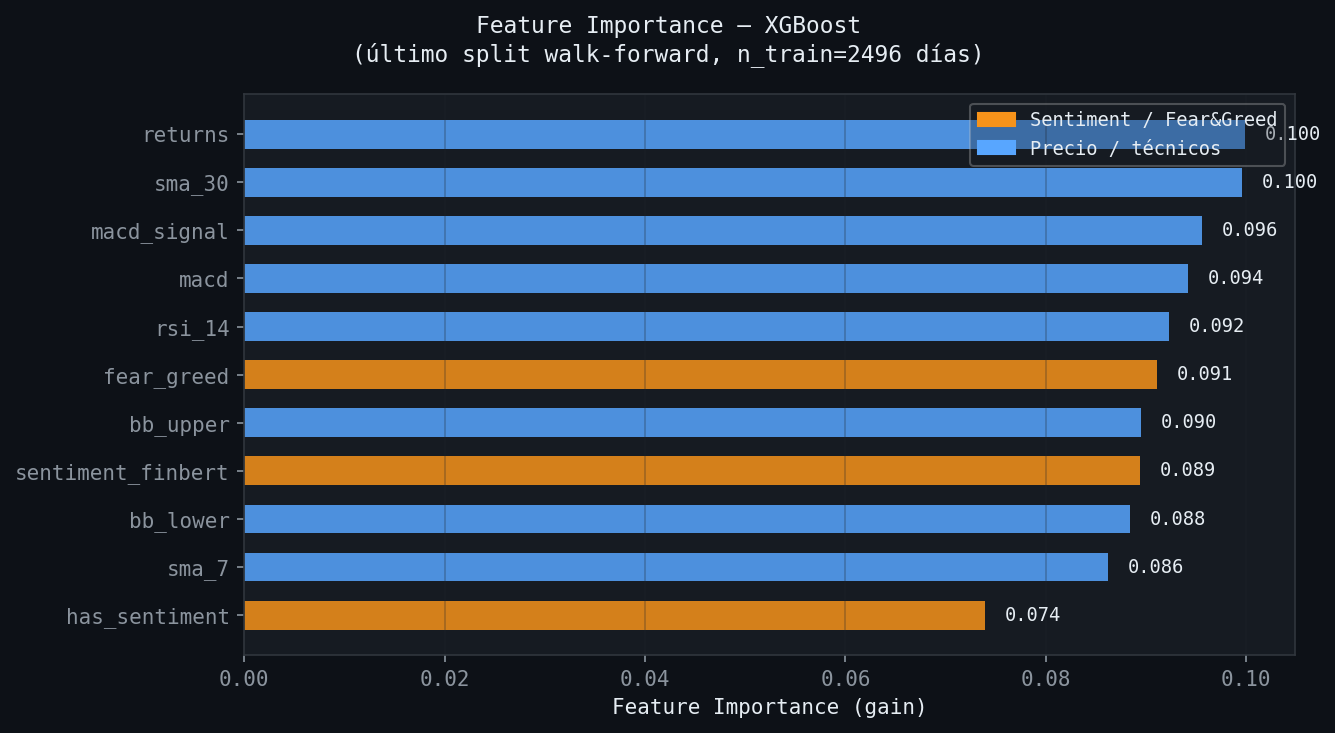
\includegraphics[width=\columnwidth]{fig06_feature_importance}
\caption{Importància relativa de les \textit{features} segons XGBoost (\textit{train}
de l'últim \textit{split}). Els retorns lideren (19,8\%) i el sentiment FinBERT
aporta $\sim$3\%; el \texttt{fear\_greed} apareix per davant de diversos indicadors
tècnics, senyal de relacions no lineals.}
\label{fig:featimp}
\end{figure}

\textbf{El sentiment no discrimina la direcció.} La prova més directa i
independent de qualsevol model és comparar la distribució del sentiment FinBERT en
dies alcistes i baixistes. El test de Mann-Whitney ($U = 821{.}316{,}5$,
$p = 0{,}342$) confirma que les distribucions són estadísticament indistingibles.
Coherentment, totes les correlacions de Pearson entre \textit{features} i
\textit{label} es mantenen per sota de $|r| = 0{,}08$ (Figura~\ref{fig:corr}). Això
no implica que les \textit{features} siguin inútils per a models no lineals: la
presència rellevant del \texttt{fear\_greed} en la importància de XGBoost confirma
que el model detecta relacions que la correlació lineal no veu.

\begin{figure}[t]
\centering
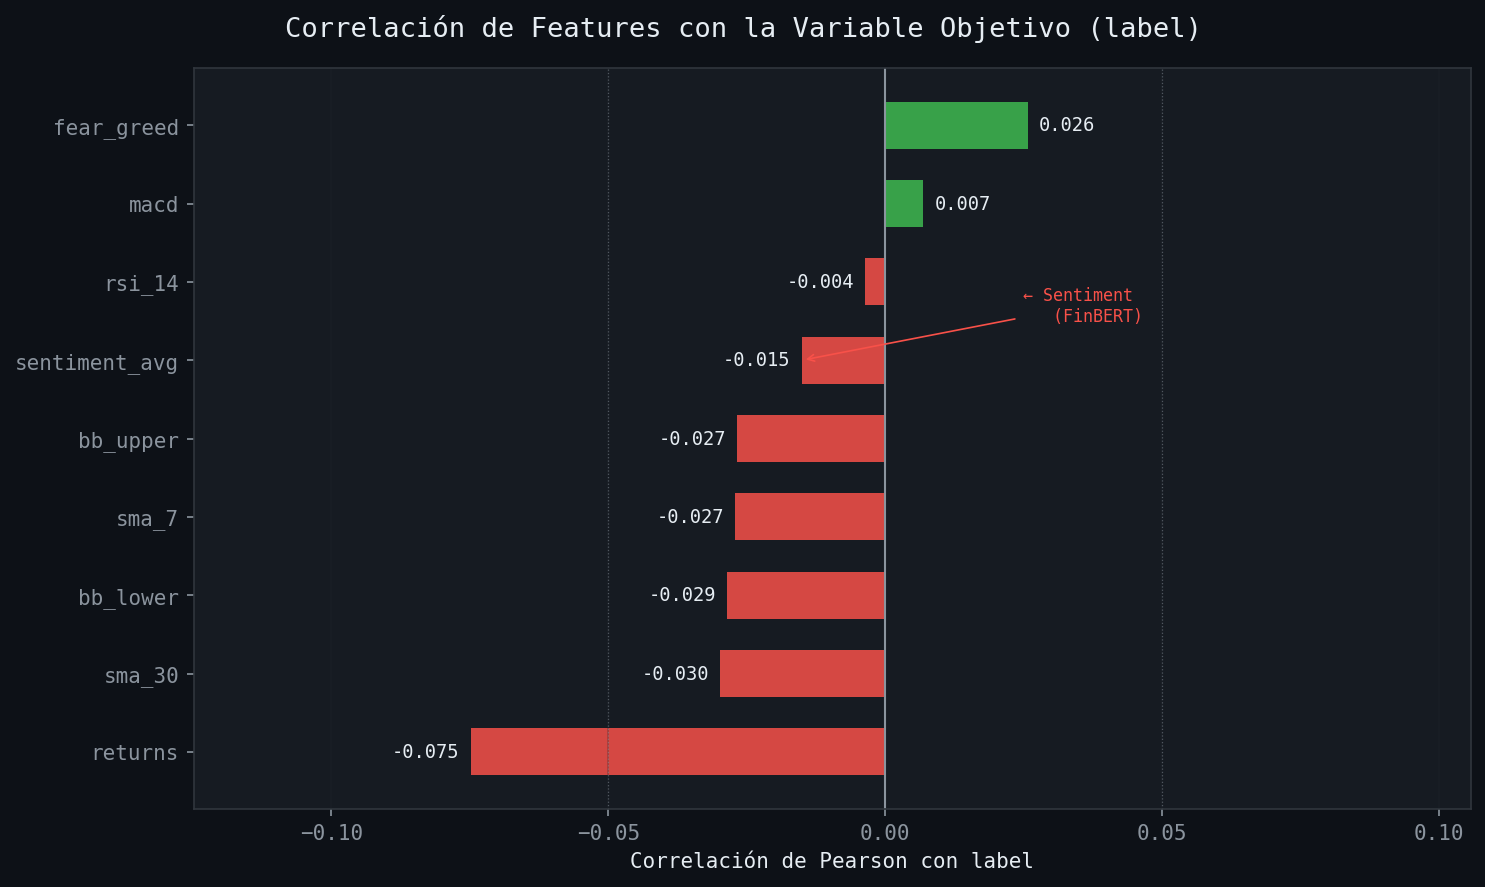
\includegraphics[width=\columnwidth]{fig03_correlacio_features}
\caption{Correlació de Pearson de cada \textit{feature} amb el \textit{label}.
Totes per sota de $|r|=0{,}08$, consistent amb l'eficiència de mercat.}
\label{fig:corr}
\end{figure}

\textbf{La dificultat és de règim, no d'algoritme.} En desglossar l'AUC per model i
\textit{split} s'observa que la dificultat es concentra en un règim de mercat
concret: el \textit{split} corresponent al període novembre--gener és
sistemàticament el pitjor en 4 dels 5 models del desglossament per \textit{split}
(Figura~\ref{fig:heatmap}, a l'apèndix), sovint per sota del 0,50. Quan
XGBoost, LightGBM i LSTM ---arquitectures molt diferents--- coincideixen en quin
\textit{split} és difícil, la constant no és el model sinó l'actiu: és una propietat
del mercat en aquell règim, no una limitació d'un algoritme particular. Aquesta
observació és rellevant perquè justifica la línia futura de models sensibles al
règim (\textit{regime-aware}).

\textbf{Causalitat inversa en el sentiment.} Per entendre per què el sentiment no
ajudava, es va dissenyar un experiment específic. L'experiment compara
\texttt{sentiment\_morning} (articles publicats abans de les 18:00 UTC) amb
\texttt{sentiment\_full} (totes les notícies del dia). La hipòtesi és que les
notícies de la tarda-nit \emph{descriuen} el moviment ja ocorregut en lloc
d'\emph{anticipar} l'endemà. La variant matinal supera la completa en 3 dels 4
\textit{splits} (Taula~\ref{tab:morning}), amb una millora mitjana
$\Delta\text{AUC} = +0{,}033$ (Figura~\ref{fig:morning}), en la direcció predita.
Cal ser honest amb la potència estadística: sota H0 (binomial $p=0{,}5$), observar
3 o més \textit{splits} en la direcció predita té probabilitat del 31,25\%
($5/16$); amb $n=4$, cap test aparellat assoleix significança. El resultat es
presenta, doncs, com a \emph{evidència direccional consistent amb la hipòtesi}, no
com a prova concloent. El seu valor és metodològic: en la literatura
de \textit{sentiment analysis} financer rarament es desagrega el sentiment per hora
del dia ---gairebé tots els estudis usen agregats diaris sense preguntar-se quines
notícies anticipen el moviment i quines el descriuen un cop ja ha passat. Aquest
experiment aporta evidència empírica que part del senyal aparent del sentiment en
estudis diaris pot ser, de fet, un artefacte de causalitat inversa: si les notícies
de la tarda-nit descriuen el que ja ha passat, incloure-les ``contamina'' l'agregat
amb informació que, per construcció, no podria anticipar res.

\begin{table}[t]
\centering
\caption{AUC per \textit{split}: sentiment matinal vs.\ complet.}
\label{tab:morning}
\small
\begin{tabular}{@{}lrrrr@{}}
\toprule
\textbf{Model} & \textbf{S1} & \textbf{S2} & \textbf{S3} & \textbf{S4} \\
\midrule
XGB+Morning ($<$18h UTC) & 0,535 & 0,582 & 0,482 & 0,514 \\
XGB+FinBERT complet      & 0,510 & 0,494 & 0,495 & 0,480 \\
\midrule
$\Delta$AUC (M$-$F)      & $+0{,}025$ & $+0{,}088$ & $-0{,}013$ & $+0{,}034$ \\
\bottomrule
\end{tabular}
\end{table}

\begin{figure}[t]
\centering
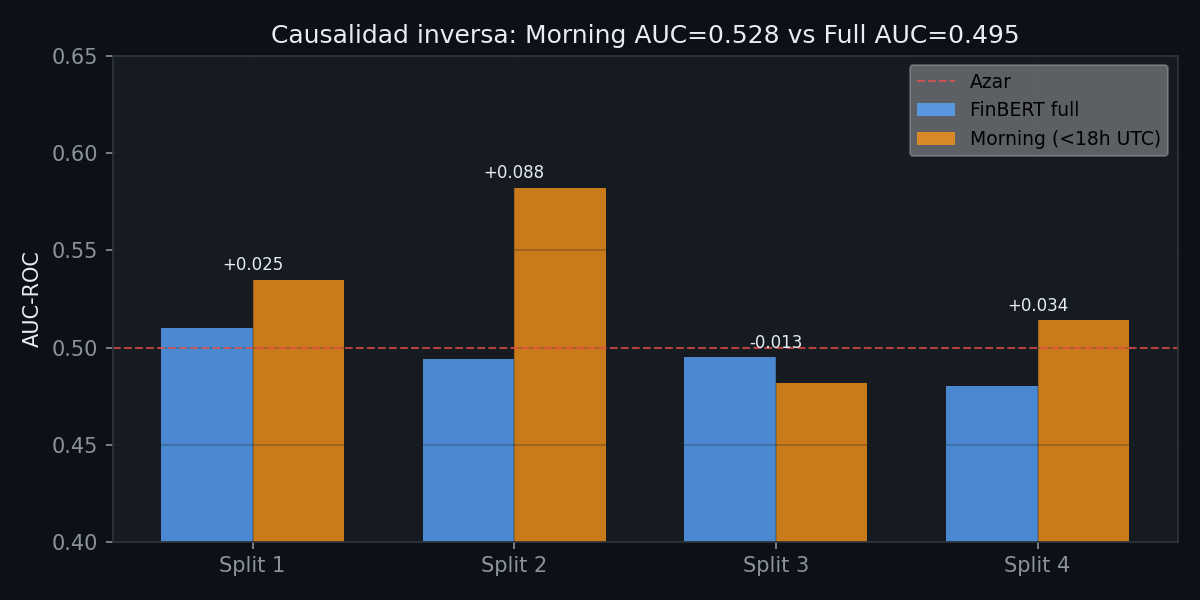
\includegraphics[width=\columnwidth]{fig09_morning_vs_full}
\caption{AUC del sentiment matinal ($<$18:00 UTC) vs.\ complet, per \textit{split}.
La variant matinal supera la completa en 3 de 4 \textit{splits}
($\Delta$AUC mitjà $=+0{,}033$).}
\label{fig:morning}
\end{figure}

\textbf{Del classificador a l'estratègia.} El \textit{backtest} del millor model
(XGBoost+Optuna; 360 dies, comissió 0,1\%) confirma l'absència de senyal des d'una
òptica de \textit{trading} (Taula~\ref{tab:backtest}). La signatura estadística
d'un model sense capacitat predictiva real és inequívoca: el Sharpe \emph{empitjora}
en augmentar el llindar de confiança ---de $-0{,}166$ a $-1{,}199$
(Figura~\ref{fig:threshold}). Si el model tingués \textit{edge}, exigir més
confiança hauria de millorar el Sharpe, no degradar-lo. L'estratègia ML perd menys
que el \textit{Buy \& Hold} només per estar fora del mercat bona part d'un període
baixista, no per encert predictiu.

La corba d'\textit{equity} confirma aquesta lectura: el \textit{drawdown} màxim
---la caiguda màxima de pic a vall, no el retorn total--- de l'estratègia ML
($-48{,}71\%$) és pràcticament igual al \textit{drawdown} del \textit{Buy \& Hold}
($-51{,}71\%$), i la petita diferència s'explica pels períodes en efectiu (43\% del
temps), no per encert en les prediccions. En altres paraules, l'única ``protecció''
que ofereix el model és no estar invertit, no anticipar les caigudes.

Convé subratllar que classificar bé i construir una estratègia rendible són
problemes diferents. Fins i tot amb el llindar per defecte el model ja opera poc més
de la meitat dels dies (56,9\% d'exposició), i exigir-li més confiança el deixa
pràcticament fora del mercat ---només un 2,2\% d'exposició al llindar 0,70
(Taula~\ref{tab:backtest})--- sense que això millori el rendiment. Una estratègia
òptima requeriria optimització del llindar, gestió dinàmica de la posició i
consciència del règim ---precisament les peces que la Fase 2 intenta articular al
voltant d'un model que, per si sol, no és fiable.

\begin{table}[t]
\centering
\caption{\textit{Backtest} XGBoost+Optuna per llindar (360 dies, comissió 0,1\%; retorn total del B\&H $=-17{,}83\%$). ``Retorn ML'' és el retorn total de l'estratègia, no el \textit{drawdown}.}
\label{tab:backtest}
\small
\setlength{\tabcolsep}{4pt}
\begin{tabular}{@{}rrrrr@{}}
\toprule
\textbf{Llindar} & \textbf{Ops} & \textbf{\% mercat} & \textbf{Retorn ML} & \textbf{Sharpe} \\
\midrule
0,50 & 69 & 56,9\% & $-13{,}26\%$ & $-0{,}166$ \\
0,55 & 29 & 16,7\% & $-10{,}46\%$ & $-0{,}216$ \\
0,60 & 15 &  8,3\% & $-19{,}53\%$ & $-0{,}734$ \\
0,65 & 15 &  6,1\% & $-24{,}01\%$ & $-1{,}199$ \\
0,70 &  6 &  2,2\% & $-17{,}81\%$ & $-0{,}967$ \\
\bottomrule
\end{tabular}
\end{table}

\begin{figure}[t]
\centering
\includegraphics[width=\columnwidth]{fig14_threshold}
\caption{Sharpe i exposició al mercat per llindar de decisió. El Sharpe empitjora
en pujar el llindar: la signatura d'un model sense senyal predictiva real.}
\label{fig:threshold}
\end{figure}

\textbf{Per què tants resultats positius del camp no es repliquen.} El cas d'aquest
treball ---un AUC aparent de 0,73 que semblava prometedor i que, un cop neta la
metodologia, va caure a un honest 0,52 indistingible de l'atzar (el cas de
\textit{leakage} del model \textit{ensemble} integrat a l'agent, detallat a la
Taula~\ref{tab:iteracions})--- no és una anomalia, sinó el patró habitual del sector. Bona part de la literatura i, sobretot,
del material divulgatiu sobre \textit{trading} algorítmic reporta sistemes que
``funcionen'' i que, en ser replicats amb una metodologia correcta, no superen
l'atzar~\cite{sebastiao2021}. Les causes són recurrents i totes elles inflen artificialment les mètriques:
\textit{data leakage} i \textit{look-ahead bias} (usar informació que en producció no
existiria, com la \textit{forward window} en les \textit{features} ICT que aquest
mateix treball va haver de corregir), validació creuada estàndard en lloc de
\textit{walk-forward} (que barreja futur i passat), absència de tests de significança
(reportar un AUC de 0,55 com a ``positiu'' sense interval de confiança),
\textit{backtests} sense costos de transacció ni \textit{slippage}, i
\textit{overfitting} per cerca repetida d'hiperparàmetres sobre el mateix conjunt de
test. El resultat és un biaix de publicació evident: els negatius rarament es
publiquen i els positius rarament es repliquen. Aquest treball inverteix
deliberadament la prioritat ---primer la metodologia, després el número--- i és
precisament aquesta disciplina la que fa que el seu resultat nul sigui més valuós que
molts positius no contrastats.

% ============================================================
\section{Sistema multi-agent d'IA}
% ============================================================
La conclusió honesta de la Fase 1 ---AUC $\approx 0{,}52$ amb IC que inclouen el
0,5--- obre una pregunta estratègica: com aprofitar una infraestructura completa
quan els models per si sols no superen l'atzar? La resposta, alineada amb la
literatura recent~\cite{stockbench2025}, és deliberadament conservadora: un model
amb AUC $\approx 0{,}5$ és inusable com a oracle autònom, però pot ser una
\emph{font de senyal feble} dins d'un sistema d'investigació més ampli que combini
mòduls heterogenis, ponderi cada senyal pel seu \textit{edge} empíric i comuniqui
explícitament la incertesa. La tesi del disseny és que un agent d'IA financera honest no és el que aspira a
substituir el judici humà, sinó el que estructura el procés de presa de decisions,
exposa les seves fonts i quantifica els seus dubtes: l'AUC del model ML és un dels
\textit{inputs} del sistema, no el seu \textit{output}.

L'arquitectura definitiva és el resultat d'una iteració. La versió inicial era un
únic agent que havia d'actuar alhora com a analista i com a controlador de risc, i
això produïa dos problemes recurrents: verificava malament les xifres ---arribant a
marcar com a ``error'' que el preu citat coincidís amb el de referència, una
tautologia--- i barrejava la verificació determinista (que hauria de ser codi) amb
el judici qualitatiu (que sí que és tasca d'un LLM). La separació en tres rols amb
responsabilitats estrictes va resoldre totes dues patologies; la migració de
\texttt{gpt-4o-mini} a \texttt{gpt-4o} va ser igualment necessària, perquè el model
petit ignorava de manera reincident les instruccions de no comparar preus.

\textbf{Arquitectura.} El sistema (Figura~\ref{fig:arch}) és un equip de tres
agents especialitzats sobre GPT-4o, amb responsabilitats estrictament separades.
L'\textbf{Analista} (\texttt{06\_agent.py}) genera l'anàlisi invocant 13 eines de
\textit{function calling} i recuperant notícies via RAG amb FAISS (1.996
documents). El \textbf{Risk Manager} (\texttt{critic\_agent.py}) audita l'anàlisi
combinant verificació \emph{determinista} en codi amb un contraargument
adversarial del LLM. El \textbf{Decision Maker} (\texttt{decision\_engine.py}) pren
la decisió final GO/NO-GO amb un \emph{motor de regles determinista}.

\textbf{Principi: codi verifica, LLM opina.} La decisió arquitectònica central és
la separació estricta entre verificació i opinió. Tot allò comprovable de manera
determinista ---el signe i la força del \textit{Confluence Score}, el ràtio
risc/benefici, la franja horària, els conflictes entre mòduls, la coherència del
preu citat--- es resol en codi Python. El LLM només s'encarrega del que aporta
valor genuí: el contraargument adversarial i la lectura qualitativa del risc. Així
s'eliminen d'arrel els falsos positius (el veredicte APPROVE/CAUTION/REJECT és
sortida de regles, mai text al\textperiodcentered{}lucinat). El motor de decisió,
davant els mateixos \textit{inputs}, sempre produeix la mateixa sortida ---propietat
indispensable per a la reproductibilitat. Les regles de NO-GO inclouen,
entre d'altres: $|$\textit{Confluence Score}$| < 0{,}30$, conflicte entre mòduls,
franja horària de baixa liquiditat (\textit{dead zone} 22:00--00:00 UTC), veredicte
REJECT del Risk Manager i ràtio risc/benefici net inferior a 1,5:1. Una crida final
al LLM (temperatura 0) redacta el veredicte en llenguatge natural, però amb el
GO/NO-GO ja fixat pel motor: el LLM l'explica, no el pot contradir. Si aquesta crida
falla, el sistema continua emetent el veredicte determinista amb un text de reserva,
de manera que la decisió mai depèn de la disponibilitat del model de llenguatge.

\begin{figure*}[t]
\centering
\resizebox{\textwidth}{!}{%
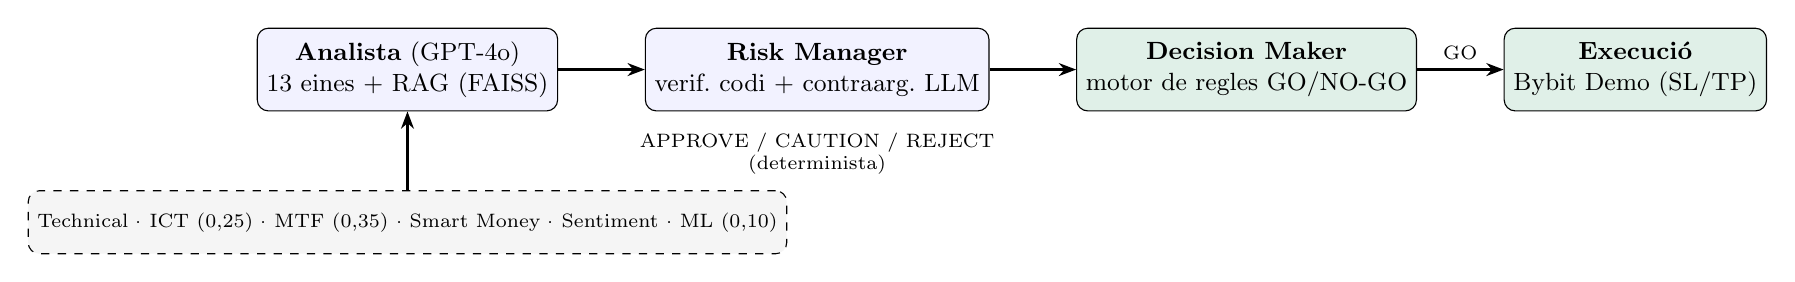
\begin{tikzpicture}[
  node distance=0.9cm and 1.1cm,
  box/.style={draw, rounded corners, align=center, minimum height=1.05cm, minimum width=2.9cm, font=\small, fill=blue!5},
  det/.style={draw, rounded corners, align=center, minimum height=1.05cm, minimum width=2.9cm, font=\small, fill=accentgreen!12},
  src/.style={draw, dashed, rounded corners, align=center, minimum height=0.8cm, font=\scriptsize, fill=gray!8},
  arr/.style={-{Stealth[length=2.2mm]}, thick},
]
\node[box] (analista) {\textbf{Analista} (GPT-4o)\\13 eines + RAG (FAISS)};
\node[box, right=of analista] (risk) {\textbf{Risk Manager}\\verif.\ codi + contraarg.\ LLM};
\node[det, right=of risk] (dec) {\textbf{Decision Maker}\\motor de regles GO/NO-GO};
\node[det, right=of dec] (exec) {\textbf{Execució}\\Bybit Demo (SL/TP)};

\node[src, below=1.0cm of analista] (sources) {Technical · ICT (0,25) · MTF (0,35) · Smart Money · Sentiment · ML (0,10)};

\draw[arr] (analista) -- (risk);
\draw[arr] (risk) -- (dec);
\draw[arr] (dec) -- node[above, font=\scriptsize] {GO} (exec);
\draw[arr] (sources) -- (analista);

\node[font=\scriptsize, below=0.15cm of risk, align=center] {APPROVE / CAUTION / REJECT\\(determinista)};
\end{tikzpicture}%
}
\caption{Arquitectura del sistema multi-agent. L'Analista sintetitza els sis mòduls
del \textit{Confluence Score} (entre ells el model ML, amb un pes del 10\%); el Risk
Manager audita amb verificació determinista; i el Decision Maker emet el GO/NO-GO amb
un motor de regles. El LLM opina, però mai pren la decisió final ni verifica xifres.}
\label{fig:arch}
\end{figure*}

\textbf{Eines i recuperació semàntica.} L'Analista disposa de 13 eines de
\textit{function calling} que cobreixen dimensions heterogènies del mercat:
indicadors tècnics, predicció del model ML (\texttt{run\_ml\_prediction}),
estructura ICT (\textit{order blocks}, \textit{fair value gaps}), \textit{bias}
multi-temporal, dades de microestructura (\textit{funding rate}, \textit{open
interest}, liquidacions), fluxos d'ETFs \textit{spot} i el càlcul del
\textit{Confluence Score}. A aquestes s'hi afegeix la recuperació semàntica: un
pipeline RAG (\texttt{rag\_pipeline.py}) amb FAISS sobre 1.996 documents
vectoritzats amb \textit{sentence-transformers} (\texttt{all-MiniLM-L6-v2}) i cerca
per similitud cosinus. El RAG fonamenta les respostes en notícies reals i en permet
la citació; quan la millor similitud és baixa ($<0{,}4$), l'eina ho declara com a
``cerca feble'', un dels mecanismes de comunicació d'incertesa.

\textbf{Mòduls de l'agent i del bot.} Cada rol i cada funció del cicle viu en un
mòdul separat, amb una frontera clara entre el que decideix i el que executa.
L'Analista (\texttt{06\_agent.py}) orquestra el bucle de \textit{function calling}
amb GPT-4o i \textit{streaming}; el Risk Manager (\texttt{critic\_agent.py}) emet el
veredicte adversarial; i el Decision Maker (\texttt{decision\_engine.py}) fusiona
\textit{Confluence Score}, veredicte de risc i paràmetres reals del \textit{trade}
(R:R, \textit{stop loss}, \textit{take profit}, \textit{sizing}) en la decisió
GO/NO-GO. L'execució es delega a un únic mòdul compartit (\texttt{trade\_executor.py})
que calcula els paràmetres, obre la posició a Bybit ---o la simula localment com a
\textit{fallback}, distingint l'ordre real de la simulada pel prefix de
l'identificador--- i la registra a la base de dades; el client de \textit{broker}
(\texttt{bybit\_client.py}) encapsula l'API de Bybit Demo. Sobre aquesta base, el bot
de \textit{paper trading} (\texttt{live\_bot.py}) opera amb un doble disparador:
horari, a l'inici de cada \textit{killzone} (Londres i Nova York), i per senyal, quan
la confluència ho justifica. Que el bot automàtic i el botó manual del
\textit{dashboard} comparteixin el mateix \texttt{trade\_executor} garanteix que tots
dos camins segueixen exactament la mateixa lògica d'execució i registre.

\textbf{Confluence Score.} L'Analista sintetitza sis mòduls de senyal en una
puntuació contínua a $[-1,+1]$, amb pesos obtinguts per \textit{grid search}
empíric sobre 22 configuracions, avaluades per retorn ajustat per risc
(Taula~\ref{tab:confluence}). És revelador que el mòdul ML rebi només un pes del
10\% ---coherent amb el seu AUC honest de 0,52--- mentre que el
\textit{multi-timeframe bias} en rep el màxim (35\%) per ser on s'observa el millor
\textit{edge} empíric. La discretització és simètrica: $\geq +0{,}30 \Rightarrow$
BUY, $\leq -0{,}30 \Rightarrow$ SELL, altrament NEUTRAL.

\begin{table}[t]
\centering
\caption{Ponderacions del \textit{Confluence Score} (config.\ \textit{Trend Following}).}
\label{tab:confluence}
\small
\begin{tabular}{@{}L{3.6cm}rL{2.4cm}@{}}
\toprule
\textbf{Mòdul} & \textbf{Pes} & \textbf{Rol} \\
\midrule
Technical    & 0,20 & base sòlida \\
ICT          & 0,25 & estructura institucional \\
\textbf{MTF} & \textbf{0,35} & \textbf{major \textit{edge}} \\
Smart Money  & 0,05 & senyal volàtil \\
Sentiment    & 0,05 & soroll a baixa freq. \\
ML           & 0,10 & AUC honest 0,52 \\
\bottomrule
\end{tabular}
\end{table}

\textbf{Una auditoria més: \textit{leakage} en el model integrat.} El mateix hàbit
de revisió va tornar a actuar en integrar el model com a eina de l'agent, quan una
versió va reportar un AUC aparentment espectacular de $0{,}728$. En lloc d'acceptar
el número, es va inspeccionar el codi: \texttt{detect\_order\_blocks} usava +50
barres futures (\emph{forward window}) per validar la persistència d'un
\textit{order block}, mentre que el \textit{target} era el moviment a +4 hores ---és
a dir, la \textit{feature} mirava un futur que en producció no existeix. Aplicat el
\texttt{shift} temporal correcte, l'AUC honest va caure a $0{,}519$, per sota fins i
tot del rang 0,55--0,65 que reporta la literatura cripto, sovint sense auditories
equivalents. Aquesta troballa documenta com un mecanisme aparentment
inofensiu (mirar endavant per confirmar un patró) pot inflar les mètriques fins a
fer un model semblar \textit{state of the art}. La Taula~\ref{tab:iteracions}
resumeix les tres iteracions del model integrat: la versió corregida (v3) és la
desplegada en producció.

\begin{table}[t]
\centering
\caption{Iteracions del model ML \textit{ensemble} integrat a l'agent.}
\label{tab:iteracions}
\small
\begin{tabular}{@{}L{2.4cm}cL{3.0cm}@{}}
\toprule
\textbf{Iteració} & \textbf{AUC} & \textbf{Estat} \\
\midrule
v1 inicial          & 0,599 & \textit{mismatch} de \textit{runtime} \\
v2 reentrenat       & 0,728 & \textbf{\textit{leakage} no detectat} \\
\textbf{v3 (post-auditoria)} & \textbf{0,519} & \textcolor{accentgreen}{\textbf{honest}} \\
\bottomrule
\end{tabular}
\end{table}

\textbf{Comunicació d'incertesa.} L'agent no presenta cap resposta sense
qualificar-ne la incertesa, mitjançant cinc mecanismes complementaris:
\begin{enumerate}[leftmargin=1.1em,itemsep=1pt,topsep=2pt]
  \item \textbf{Confiança del \textit{Confluence Score}}: nivell qualitatiu
  (alta / mitjana / baixa) que el \textit{prompt} obliga a citar en cada
  recomanació direccional.
  \item \textbf{\textit{Conflict flag}}: si el sentiment i l'estructura (ICT+MTF)
  divergeixen, l'eina emet un avís i recomana reduir la mida de posició a la meitat.
  \item \textbf{Fallades d'eines}: si una eina retorna error o dades insuficients,
  l'agent ho declara explícitament en lloc d'inventar valors.
  \item \textbf{Qualitat del RAG}: si la millor similitud és $<0{,}4$, la cerca
  s'etiqueta com a feble i s'adverteix que el context pot no ser representatiu.
  \item \textbf{Recordatori de limitacions}: cada resposta inclou un breu recordatori
  (mida del corpus, dependència de \textit{killzones} ICT, AUC honest $\approx 0{,}52$).
\end{enumerate}
És, en termes pràctics, una \emph{calibració procedimental}: en lloc de calibrar
les probabilitats d'un classificador sense poder predictiu, es calibra el
llenguatge de l'agent perquè reflecteixi la qualitat dels seus \textit{inputs}.

\textbf{Avaluació empírica.} El sistema complet s'avalua per quatre vies
complementàries, cadascuna dirigida a un component diferent
(Taula~\ref{tab:mapaeval}). El sistema RAG s'avalua amb un \textit{framework}
inspirat en RAGAS~\cite{es2024} sobre 20 preguntes en 5 categories.

\begin{table}[t]
\centering
\caption{Mapa d'avaluació del sistema complet.}
\label{tab:mapaeval}
\small
\begin{tabular}{@{}L{2.2cm}L{2.7cm}L{2.6cm}@{}}
\toprule
\textbf{Component} & \textbf{Mètode} & \textbf{Resultat clau} \\
\midrule
Models ML & Walk-forward 4$\times$90 & AUC 0,532 (\textit{ns}) \\
Estratègia & \textit{Backtest} 360 dies & Sharpe empitjora amb el llindar \\
RAG agent & RAGAS (20 preg.) & \textit{Faithfulness} 0,863 \\
LLM filtre & Ablació 365 dies & $-4{,}5\%$ en \textit{bear} \\
\bottomrule
\end{tabular}
\end{table} El resultat
més destacable és un \textbf{\textit{Faithfulness} de 0,863}, per sobre del llindar
industrial de 0,75: les respostes estan ben fonamentades en el context recuperat,
sense al\textperiodcentered{}lucinacions significatives (\textit{Answer Relevancy}
0,658, \textit{Context Precision} 0,611, més baixos per limitacions
d'\textit{embeddings} monolingües i respostes ML sense passatges de context;
Taula~\ref{tab:ragas}). La
categoria Macro, amb \textit{Faithfulness} de $0{,}00$ abans del RAG, assoleix
$1{,}00$ després: abans de la integració del RAG l'agent no podia respondre
preguntes macroeconòmiques perquè cap eina estructurada cobria aquest domini, i la
transició $0{,}00 \to 1{,}00$ és evidència directa que la cerca semàntica aporta
cobertura informativa que les eines estructurades no poden replicar. Un estudi
d'ablació LLM (\textit{backtest}
de 365 dies, 500 crides reals) dona un \textit{null finding} addicional: usar el
LLM com a filtre final \emph{empitjora} el retorn un 4,5\% en una fase baixista
perllongada, perquè els criteris ICT estrictes descarten operacions guanyadores.
\begin{table}[t]
\centering
\caption{Resultats RAGAS (20 preguntes, 5 categories).}
\label{tab:ragas}
\small
\begin{tabular}{@{}L{3.4cm}rr@{}}
\toprule
\textbf{Mètrica} & \textbf{Score} & \textbf{Llindar prod.} \\
\midrule
\textbf{Faithfulness} & \textbf{0,863} & $\geq 0{,}75$ \\
Answer Relevancy      & 0,658          & $\geq 0{,}80$ \\
Context Precision     & 0,611          & $\geq 0{,}70$ \\
\bottomrule
\end{tabular}
\end{table}

El resultat coincideix qualitativament amb StockBench~\cite{stockbench2025} (``most
LLM agents struggle to outperform a simple buy-and-hold in extended trending
periods'') i obre la línia del \emph{regime-aware prompting}.

Una limitació metodològica fonamental afecta qualsevol \textit{backtest} històric
amb LLMs: el model conté coneixement paramètric del període avaluat, i encara que
el RAG filtri temporalment els documents, no es pot filtrar aquest coneixement
intern ---un soroll \textit{look-ahead} impossible d'eliminar retrospectivament. Per
això, l'única avaluació plenament neta de l'agent és la prospectiva: el
\textit{paper trading} en viu. Quan la decisió és GO, el sistema habilita l'execució
directa sobre el compte de pràctiques de Bybit, amb un \textit{gating} verificat al
servidor (només executa si la decisió és GO i no ha caducat). L'execució i el
registre es centralitzen en un únic mòdul compartit pel bot automàtic i pel botó
manual, que obre la posició amb \textit{stop loss} i \textit{take profit} natius i la
registra a la base de dades. La gestió posterior incorpora \textit{break-even} i
\textit{trailing stop}: en arribar a un benefici llindar, el \textit{stop loss} es
desplaça a l'entrada (la posició ja no pot perdre) i després segueix el preu ---una
protecció que persisteix al \textit{broker} encara que el bot s'apagui. Aquesta
infraestructura constitueix la línia de continuació prioritària.

Al tancament del període documentat, tots els components del sistema estan operatius:
les 13 eines de \textit{function calling}, el bucle conversacional amb GPT-4o i
\textit{streaming} SSE, el sistema multi-agent complet, el motor de decisió
determinista, el pipeline RAG amb FAISS i el model ML auditat (v3). Tota aquesta
maquinària arriba a l'usuari a través d'un \textit{dashboard} web, que es descriu a
continuació.

% ============================================================
\section{Dashboard i visualització}
% ============================================================
Perquè un sistema d'aquesta complexitat sigui interpretable ---i defensable--- cal
una capa de presentació que en faci visibles les decisions i les seves fonts. El
\textit{dashboard} web (Figura~\ref{fig:dashboard}), construït amb Flask i
\textit{TradingView Lightweight Charts}, segueix una separació estricta entre
\textit{frontend} (només presentació) i \textit{backend} (totes les dades), que
exposa \textbf{18 \textit{endpoints} REST} amb polítiques de \textit{refresh}
diferenciades (preu \textit{live} cada segon, gràfic cada 60\,s, la resta cada
30\,s). El contingut s'organitza en \textbf{8 pestanyes}: quatre visibles
---\emph{Senyals} (les barres dels sis mòduls del \textit{Confluence Score} i els
nivells tècnics amb R:R), \emph{Agente IA} (el botó d'anàlisi que retorna en
\textit{streaming} SSE la sortida de l'agent), \emph{Bot} (mètriques, \textit{equity
curve} i històric de \textit{trades}) i \emph{Notícies}--- i quatre més en un
\textit{dropdown} (\emph{Resumen}, \emph{Sentiment}, \emph{Sistema} ---amb les
mètriques de transparència de l'agent, RAG i RAGAS--- i \emph{Educació}). Aquesta
darrera pestanya és la més diferencial: explica amb llenguatge planer els deu
conceptes ICT (\textit{order block}, \textit{fair value gap}, \textit{killzones}\dots)
que el sistema utilitza, de manera que un avaluador no especialitzat en
\textit{trading} pugui jutjar les decisions sense bibliografia externa. El botó
d'execució del panell i el bot automàtic comparteixen el mateix mòdul d'execució, de
manera que el que es veu al \textit{dashboard} és exactament el que opera contra el
\textit{broker}.

\begin{figure}[t]
\centering
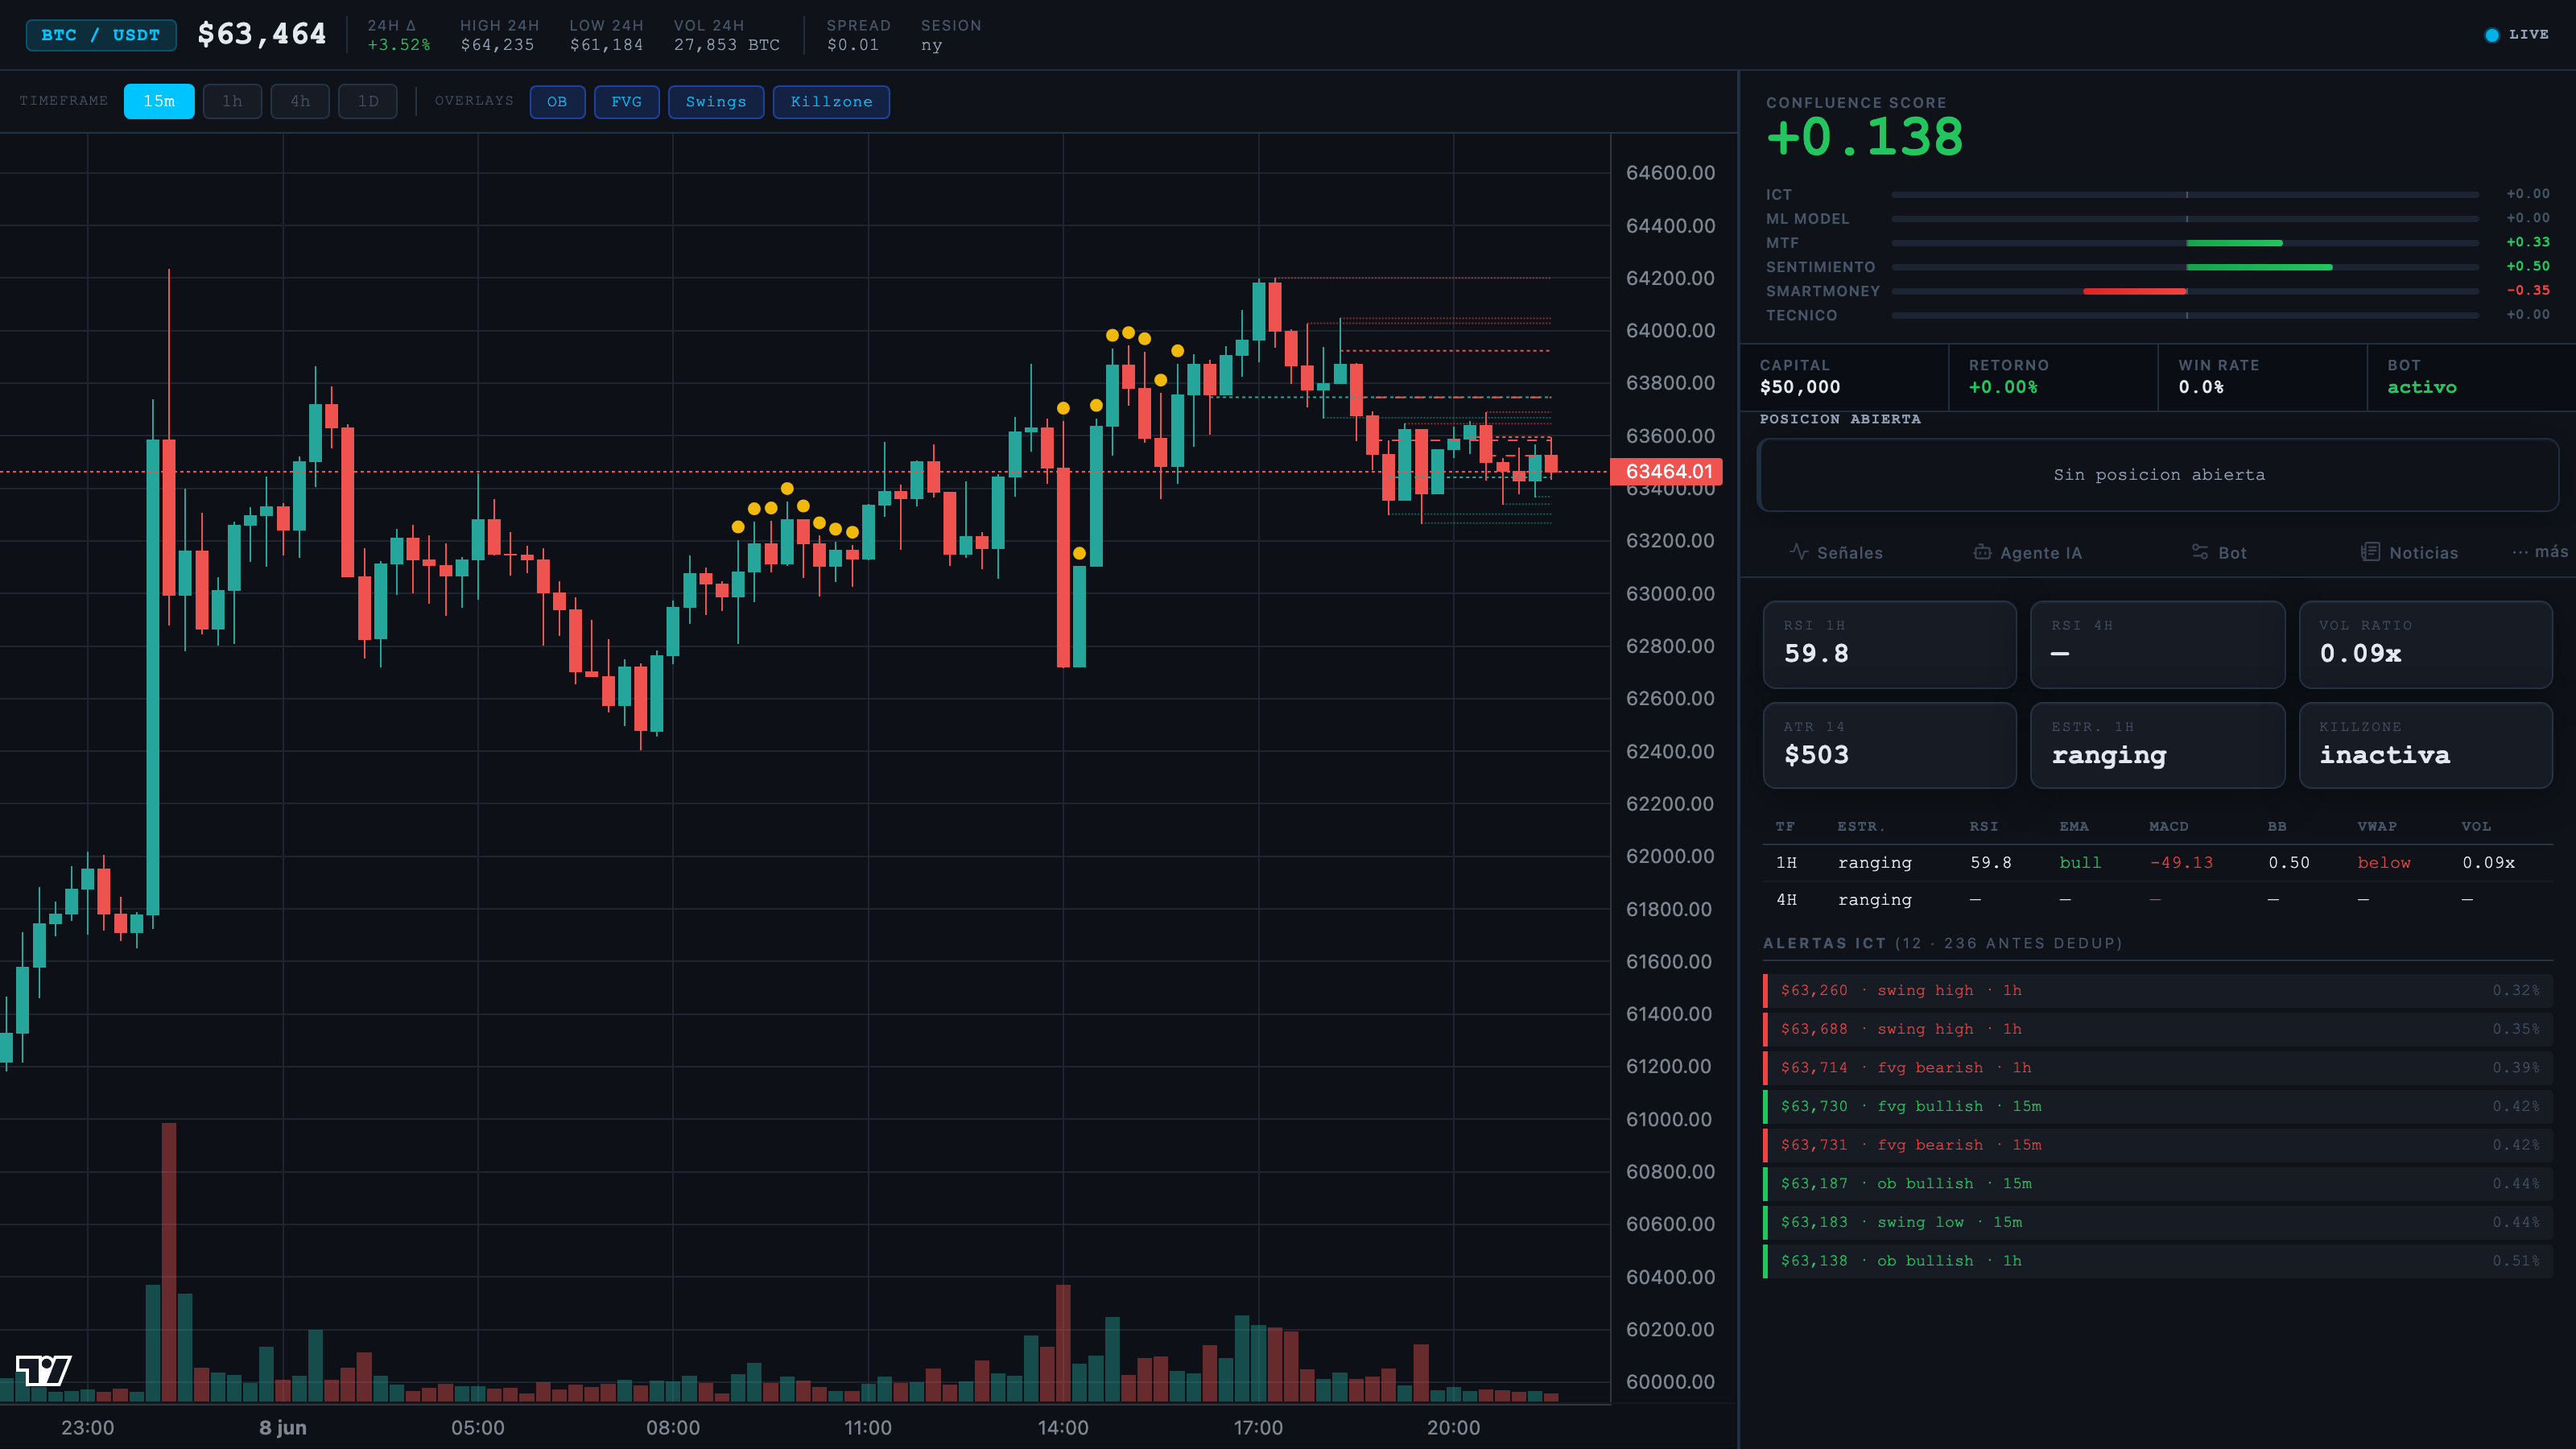
\includegraphics[width=\columnwidth]{fig_dashboard_general}
\caption{\textit{Dashboard} web (Flask + TradingView Lightweight Charts) que
integra el senyal de l'agent, els mòduls de \textit{confluence} i l'estat del bot
de \textit{paper trading}.}
\label{fig:dashboard}
\end{figure}

% ============================================================
\section{Conclusions}
% ============================================================
El treball partia d'una pregunta concreta i, després d'una avaluació
deliberadament rigorosa, la resposta és \textbf{no}: cap de les quatre famílies de
models supera l'atzar de manera significativa (millor AUC $= 0{,}532$;
$p = 0{,}287$; IC95\% que inclou el 0,5), i l'estratègia derivada perd diners amb
costos realistes, amb un Sharpe que empitjora en exigir més confiança. El resultat
és consistent amb la forma semi-forta de la HEM per a un actiu líquid en horitzó
diari. Lluny de ser un fracàs, aquest \textit{null finding} verificat val més que
un positiu que ningú no ha contrastat.

Tres contribucions donen unitat al treball sota un mateix fil ---distingir el
senyal real de l'artefacte. \textbf{(1)} Una infraestructura de dades completa i
reproduïble (PostgreSQL amb 12 taules, 105.125 notícies, 65.466 OHLCV, pipeline
diari). \textbf{(2)} El \textit{null finding} explicat per dos resultats originals:
l'auditoria de \textit{leakage} (AUC aparent $0{,}73 \to 0{,}52$ honest en corregir
una \textit{forward window}) i l'experiment de causalitat inversa (el sentiment
matinal és més informatiu que l'agregat diari). Tots dos mostren \emph{per què}
apareixen els positius espuris del camp. \textbf{(3)} Un sistema multi-agent honest
que reutilitza el model com a senyal feble (10\%) dins d'un disseny on la decisió
final la pren un motor de regles, no el LLM, i que comunica la seva incertesa en
lloc d'ocultar-la.

Aquestes contribucions són el resultat d'un procés iteratiu de diversos mesos:
d'una infraestructura inicial de quatre taules i dades de preu, a una primera etapa
de modelatge amb resultats aparentment positius, l'ampliació del corpus i
l'auditoria que els va desautoritzar, i finalment la transició cap a l'agent ---primer
únic, després multi-agent. En cada fase la temptació era acceptar el resultat
afalagador; la decisió, a cada fase, va ser verificar-lo i, sovint, desautoritzar-lo.
La Taula~\ref{tab:compliment} contrasta cada objectiu específic amb l'evidència
aportada: tots s'han assolit, atès que es van formular com a objectius de recerca i
construcció, no com la garantia d'un model rendible.

\begin{table}[t]
\centering
\caption{Compliment dels objectius específics.}
\label{tab:compliment}
\small
\begin{tabular}{@{}lL{5.3cm}l@{}}
\toprule
\textbf{OE} & \textbf{Evidència} & \textbf{Estat} \\
\midrule
OE1 & BD de 12 taules + pipeline diari & \textcolor{accentgreen}{\textbf{Assolit}} \\
OE2 & Corpus de 105.125 textos, cobertura 96,2\% & \textcolor{accentgreen}{\textbf{Assolit}} \\
OE3 & 4 famílies amb \textit{walk-forward} + IC95\% & \textcolor{accentgreen}{\textbf{Assolit}} \\
OE4 & Mann-Whitney $p=0{,}342$ + causalitat inversa & \textcolor{accentgreen}{\textbf{Assolit}} \\
OE5 & 10 problemes corregits + \textit{leakage} ICT & \textcolor{accentgreen}{\textbf{Assolit}} \\
OE6 & Multi-agent + \textit{dashboard} + bot a Bybit & \textcolor{accentgreen}{\textbf{Assolit}} \\
OE7 & RAGAS: \textit{Faithfulness} 0,863 (20 preg.) & \textcolor{accentgreen}{\textbf{Assolit}} \\
\bottomrule
\end{tabular}
\end{table}

Cal separar dues afirmacions que sovint es confonen: que un sistema \emph{funcioni}
com a enginyeria i que es pugui \emph{demostrar que és rendible}. El sistema
multi-agent està construït i verificat per vies independents (RAGAS
\textit{Faithfulness} 0,863; auditoria del \textit{leakage}; validació
extrem-a-extrem del cicle, amb un primer \textit{trade} pilot obert, gestionat i
tancat correctament en viu). Ara bé, la seva rendibilitat \textbf{no és demostrable
encara}: l'evidència de retorn disponible correspon a configuracions anteriors (el
\textit{backtest} del model sense LLM perd diners; l'ablació de l'agent únic
empitjora un 4,5\% en \textit{bear}), el sistema actual no s'ha avaluat sobre
retorn i, per construcció, no es pot \textit{backtestejar} sense contaminació
\textit{look-ahead}. Un sol \textit{trade} guanyador és estadísticament
indistingible de l'atzar; presentar-lo com a prova de rendibilitat seria l'error
que aquest treball denuncia. Tenim, doncs, una prova pilot reeixida i una pregunta
oberta que només l'avaluació en viu prolongada podrà tancar.

\textbf{Limitacions.} La limitació més important és que \emph{no s'ha pogut completar
la validació estadística de la rendibilitat} del sistema final, i convé ser explícit
sobre per què. Primera, la \emph{potència estadística} de la fase predictiva: amb
només 4 \textit{splits} de 90 dies els intervals de confiança són amplis i cap test
pot detectar efectes febles ---és, de fet, una de les raons per les quals els
resultats són nuls i no concloents en sentit fort. Segona, i més determinant,
\textit{backtestejar} un agent basat en un LLM introdueix soroll difícil de
controlar: el model arrossega coneixement paramètric del període avaluat, de manera
que sobre dades històriques té un accés implícit al futur que impedeix aïllar una
senyal neta i fa inviable un \textit{backtest} realment net. Tercera, l'\emph{horitzó
temporal} de la prova en viu és encara massa curt per extreure'n conclusions
estadístiques. Cap d'aquestes limitacions invalida el sistema com a peça
d'enginyeria; el que fan és acotar què se'n pot afirmar avui i assenyalar que només
l'avaluació prospectiva podrà tancar la qüestió de la rendibilitat.

\textbf{Línies futures.} D'aquestes limitacions se'n deriven les prioritats:
(i) augmentar la potència estadística treballant amb dades horàries o de 4~h
($n>50$ \textit{splits}); (ii) introduir models sensibles al règim de mercat i
\emph{regime-aware prompting}, ajustant la restrictivitat dels criteris ICT segons
el règim detectat; (iii) granular el sentiment per hora, font i categoria temàtica;
(iv) ampliar el \textit{test set} de RAGAS i incorporar un segon LLM-jutge; i
(v) estendre l'avaluació prospectiva del bot durant un període prou llarg per
contrastar la rendibilitat amb significança.

L'aprenentatge més important no és tècnic sinó epistemològic: en \textit{machine
learning} financer, la dificultat real no és entrenar models ---qualsevol pot
obtenir un AUC de 0,73--- sinó assegurar-se que el número reportat és real. Aquest
rigor és el fil que uneix les dues fases del projecte: és el mateix que va fer caure
l'AUC de 0,73 a 0,52 en corregir el \textit{leakage}, el que va revelar la
causalitat inversa del sentiment, i el que impedeix presentar un grapat
d'operacions guanyadores com una prova de rendibilitat. En finances quantitatives,
l'honestedat metodològica no és un afegit ètic, sinó la condició mateixa de la
validesa dels resultats.

% ============================================================
\section*{Agraïments}
% ============================================================
L'autor agraeix al tutor del TFG l'orientació metodològica, i a la comunitat
\textit{open-source} les eines que han fet possible un projecte d'aquest abast amb
un cost pràcticament nul.

% ============================================================
\begin{thebibliography}{99}
\small
\bibitem{fama1970} E.~F. Fama, ``Efficient Capital Markets: A Review of Theory and Empirical Work,'' \textit{The Journal of Finance}, vol.~25, no.~2, pp.~383--417, 1970.
\bibitem{liu2020} Y.~Liu et al., ``FinBERT: A Pre-trained Financial Language Representation Model for Financial Text Mining,'' in \textit{Proc. IJCAI}, 2020.
\bibitem{fischer2018} T.~Fischer and C.~Krauss, ``Deep learning with long short-term memory networks for financial market predictions,'' \textit{European Journal of Operational Research}, vol.~270, no.~2, pp.~654--669, 2018.
\bibitem{sezer2020} O.~B. Sezer, M.~U. Gudelek, and A.~M. Ozbayoglu, ``Financial time series forecasting with deep learning: A systematic literature review,'' \textit{Applied Soft Computing}, vol.~90, p.~106074, 2020.
\bibitem{bollen2011} J.~Bollen, H.~Mao, and X.~Zeng, ``Twitter mood predicts the stock market,'' \textit{Journal of Computational Science}, vol.~2, no.~1, pp.~1--8, 2011.
\bibitem{sebastiao2021} H.~Sebastião and P.~Godinho, ``Forecasting and trading cryptocurrencies with machine learning under changing market conditions,'' \textit{Financial Innovation}, vol.~7, no.~1, pp.~1--30, 2021.
\bibitem{uras2020} N.~Uras et al., ``Forecasting Bitcoin closing price series using linear regression and neural networks models,'' \textit{PeerJ Computer Science}, vol.~6, p.~e279, 2020.
\bibitem{lopezdeprado2018} M.~López de Prado, \textit{Advances in Financial Machine Learning}. Wiley, 2018.
\bibitem{es2024} S.~Es et al., ``RAGAS: Automated Evaluation of Retrieval Augmented Generation,'' in \textit{Proc. EACL}, 2024.
\bibitem{lewis2020} M.~Lewis et al., ``Retrieval-Augmented Generation for Knowledge-Intensive NLP Tasks,'' in \textit{Proc. NeurIPS}, 2020.
\bibitem{xiong2024} M.~Xiong et al., ``Can LLMs Express Their Uncertainty? An Empirical Evaluation of Confidence Elicitation in Large Language Models,'' \textit{arXiv:2306.13063}, 2024.
\bibitem{urquhart2016} A.~K. Urquhart, ``The inefficiency of Bitcoin,'' \textit{Economics Letters}, vol.~148, pp.~80--82, 2016.
\bibitem{chen2016} T.~Chen and C.~Guestrin, ``XGBoost: A Scalable Tree Boosting System,'' in \textit{Proc. ACM KDD}, pp.~785--794, 2016.
\bibitem{stockbench2025} Y.~Lin et al., ``StockBench: Can LLM Agents Trade Stocks Profitably in Real-World Markets?,'' \textit{arXiv:2510.02209}, 2025.
\bibitem{yao2023react} S.~Yao et al., ``ReAct: Synergizing Reasoning and Acting in Language Models,'' in \textit{Proc. ICLR}, 2023.
\bibitem{xiao2024tradingagents} Y.~Xiao et al., ``TradingAgents: Multi-Agents LLM Financial Trading Framework,'' \textit{arXiv:2412.20138}, 2024.
\bibitem{yu2023finmem} Y.~Yu et al., ``FinMem: A Performance-Enhanced LLM Trading Agent with Layered Memory and Character Design,'' \textit{arXiv:2311.13743}, 2023.
\bibitem{zhang2024finagent} W.~Zhang et al., ``A Multimodal Foundation Agent for Financial Trading: Tool-Augmented, Diversified, and Generalist,'' in \textit{Proc. ACM SIGKDD}, 2024.
\bibitem{du2023debate} Y.~Du, S.~Li, A.~Torralba, J.~B. Tenenbaum, and I.~Mordatch, ``Improving Factuality and Reasoning in Language Models through Multiagent Debate,'' \textit{arXiv:2305.14325}, 2023.
\end{thebibliography}

\onecolumn
\appendix

\section{Verificació de \textit{target leakage}}
El test següent es va integrar al \textit{pipeline} per garantir que l'etiqueta
codifica el dia següent i no l'actual. La correlació esperada per a BTC en horitzó
diari és lleugerament negativa (reversió a la mitjana).
\begin{lstlisting}
from scipy.stats import pearsonr

def verify_no_target_leakage(df, tolerance=(-0.1, -0.05)):
    """Verifica que label_t codifica el dia seguent, no l'actual.
    Si label_t = 1 quan Close_{t+1} > Close_t, aleshores:
      - corr(returns_t, label_t) ha de ser negativa (reversio a la mitjana)
      - El valor esperat es ~-0.07 per BTC en horitzo diari."""
    r, p = pearsonr(df['returns'], df['label'])
    assert tolerance[0] < r < tolerance[1], \
        f"Possible target leakage: r={r:.4f} fora de {tolerance}"
    print(f"OK: corr(returns, label) = {r:.4f}  (p={p:.4f})")
    return r

# Resultat: corr(returns_t, label_t) = -0.0725  OK
\end{lstlisting}

\section{Configuració \textit{walk-forward} amb \textit{gap} temporal}
La rutina de partició garanteix un \textit{embargo} de 7 dies entre \textit{train} i
\textit{test} (Figura~\ref{fig:wf-diagram}), que impedeix que les \textit{features}
amb finestra mòbil contaminin el conjunt de validació.
\begin{lstlisting}
def get_walk_forward_splits(df, n_splits=4, test_size=90, gap=7):
    """Walk-forward validation amb gap temporal (purging).
    El gap impedeix que features amb finestra movil contaminin el test.
      n_splits  : nombre de splits (4 per defecte)
      test_size : dies de test per split (90 per defecte)
      gap       : embargament entre train i test (7 dies)."""
    splits, n = [], len(df)
    for i in range(n_splits):
        test_end   = n - i * test_size
        test_start = test_end - test_size
        train_end  = test_start - gap
        if train_end <= 0:
            break
        splits.append((range(0, train_end), range(test_start, test_end)))
    return list(reversed(splits))
\end{lstlisting}

\begin{figure}[H]
\centering
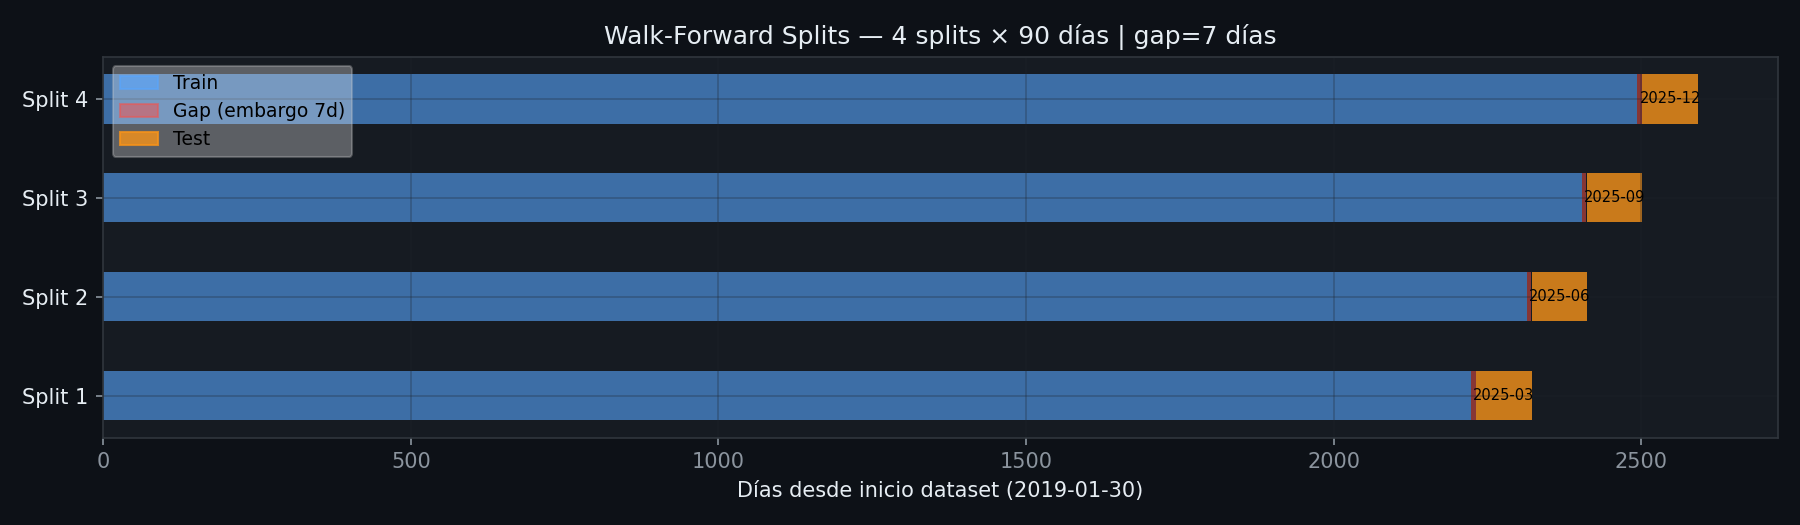
\includegraphics[width=0.78\textwidth]{fig05_walkforward}
\caption{Esquema del \textit{walk-forward validation} amb \textit{gap} temporal. Cada
\textit{split} té un \textit{train} creixent, un embargament de 7 dies i un
\textit{test} de 90 dies.}
\label{fig:wf-diagram}
\end{figure}

\section{Models: hiperparàmetres i \textit{features}}
La configuració del model XGBoost \textit{baseline} és: 300 arbres,
\texttt{max\_depth}$=3$, \texttt{learning\_rate}$=0{,}03$, regularització L1
($\alpha=0{,}1$) i L2 ($\lambda=1{,}0$). El conjunt de \textit{features} estàndard
combina indicadors tècnics (RSI-14, MACD i senyal, Bandes de Bollinger, SMA-7/30),
retorns, l'índex \textit{fear \& greed} i el sentiment FinBERT. La importància
relativa d'aquestes \textit{features} es discuteix al cos de l'article
(Figura~\ref{fig:featimp}); la Figura~\ref{fig:labeldist} en mostra l'equilibri de la
variable objectiu.

\begin{figure}[H]
\centering
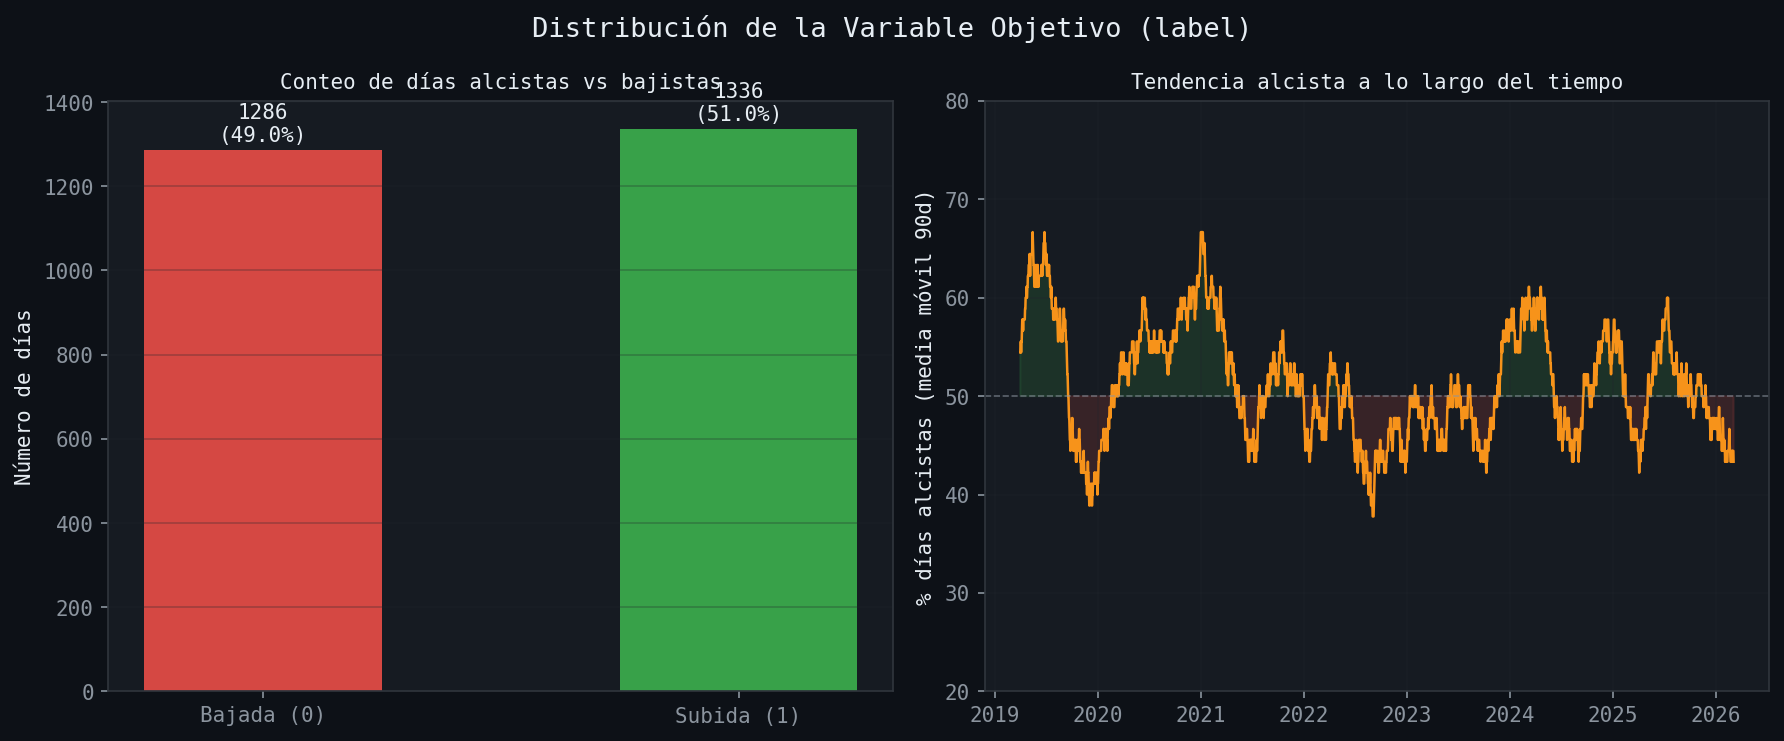
\includegraphics[width=0.6\textwidth]{fig02_distribucio_label}
\caption{Distribució de la variable objectiu: 51,0\% de dies alcistes i 49,0\%
baixistes sobre 2.711 dies (\textit{baseline} d'\textit{accuracy} 51\%).}
\label{fig:labeldist}
\end{figure}

\section{Heterogeneïtat entre \textit{splits}}
La Figura~\ref{fig:heatmap} desglossa l'AUC per model i \textit{split}: el període
novembre--gener és sistemàticament el més difícil per a arquitectures molt diferents,
fet que indica que la dificultat prové del règim de mercat i no de l'algoritme.

\begin{figure}[H]
\centering
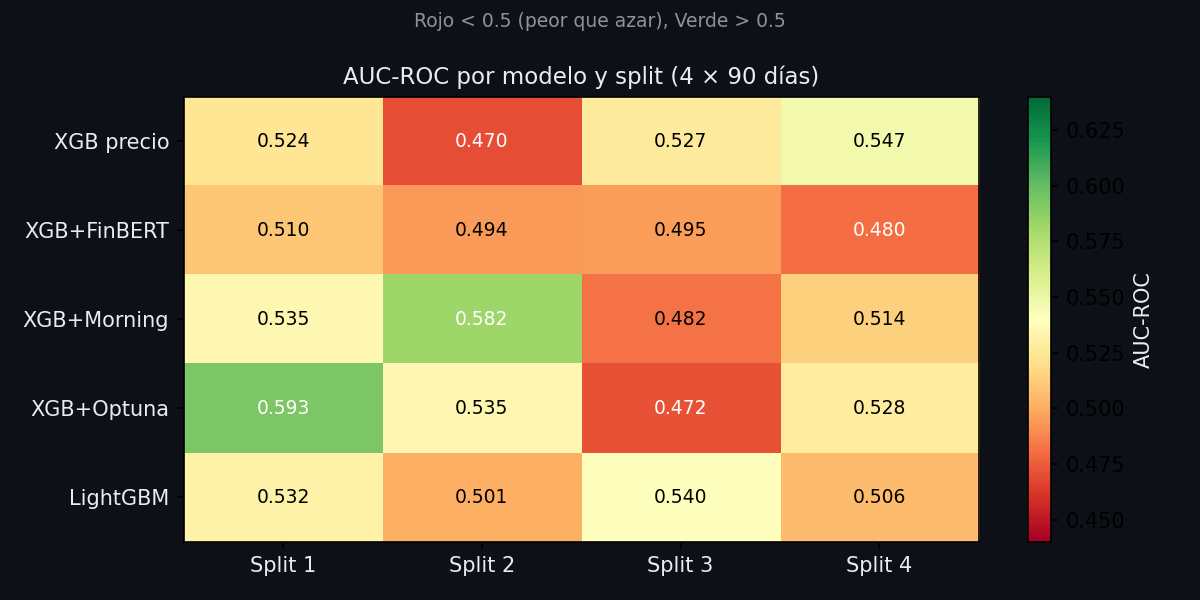
\includegraphics[width=0.72\textwidth]{fig08_auc_heatmap}
\caption{AUC per model i \textit{split}. Els valors per sota de 0,50 (pitjor que
l'atzar) es concentren en un mateix règim de mercat.}
\label{fig:heatmap}
\end{figure}

\section{Backtest: \textit{equity} i \textit{drawdown}}
Les figures següents comparen l'estratègia ML (llindar $0{,}50$) amb el
\textit{Buy \& Hold} sobre els 360 dies de test. La diferència s'explica pels
períodes en efectiu, no per capacitat predictiva.

\begin{figure}[H]
\centering
\begin{minipage}{0.49\textwidth}
  \centering
  \includegraphics[width=\textwidth]{fig12_equity_curve}
  \caption{Corba d'\textit{equity}: ML ($\theta=0{,}50$) vs.\ \textit{Buy \& Hold}.}
  \label{fig:equity}
\end{minipage}\hfill
\begin{minipage}{0.49\textwidth}
  \centering
  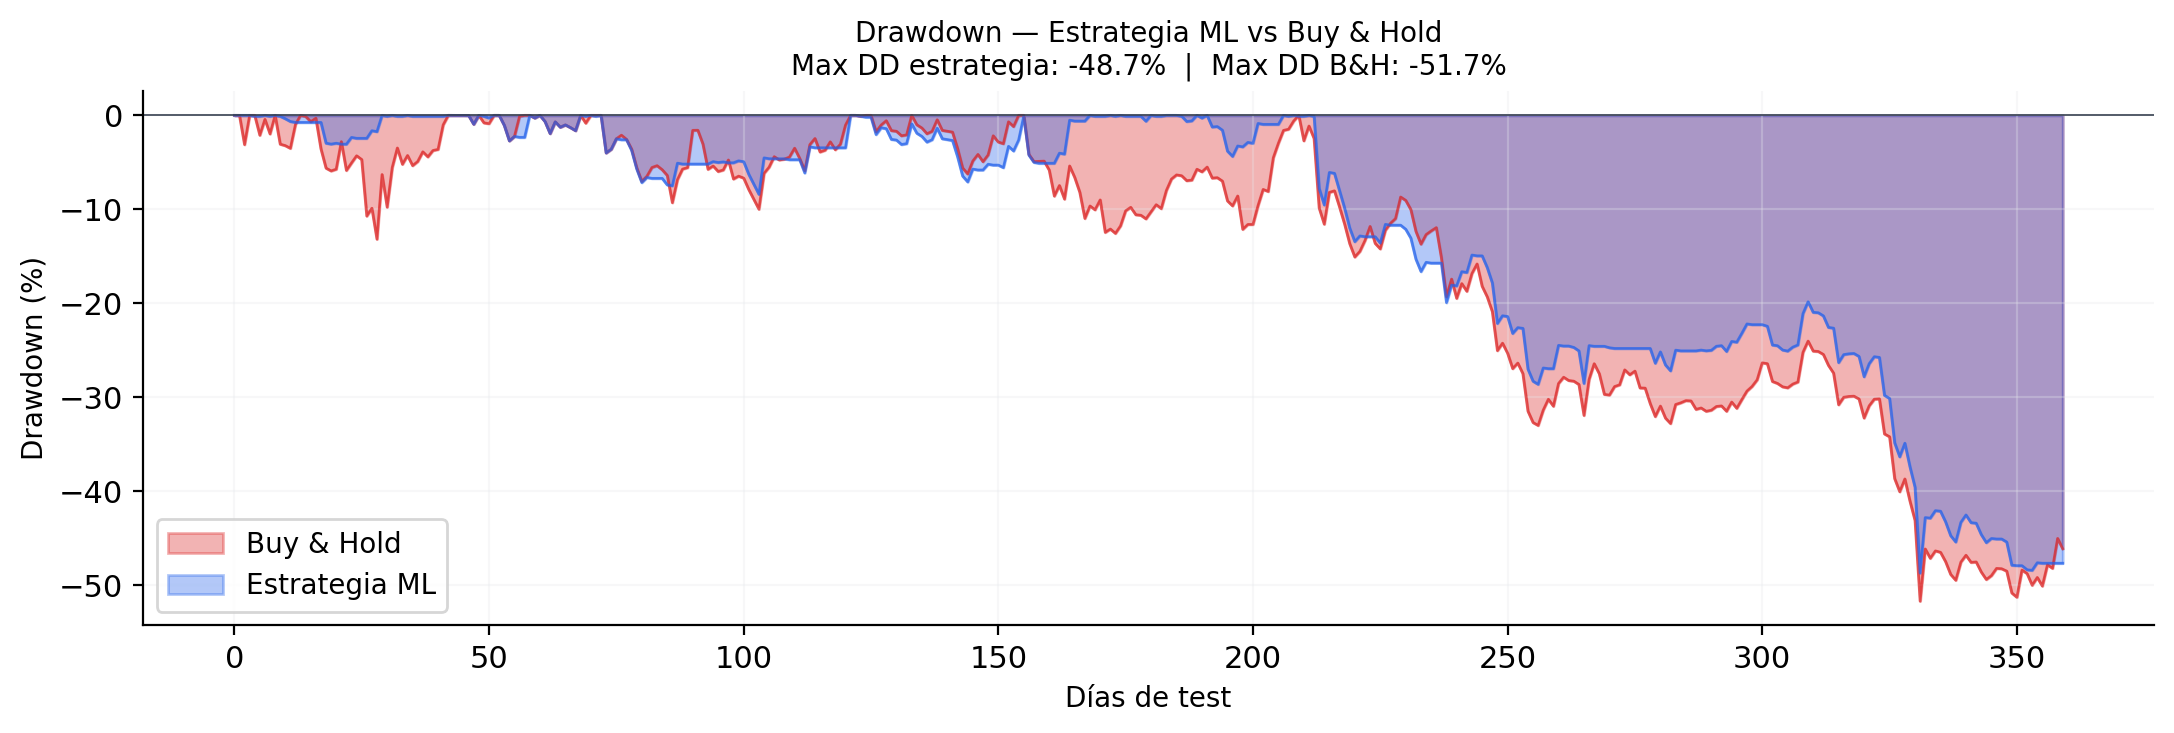
\includegraphics[width=\textwidth]{fig13_drawdown}
  \caption{\textit{Drawdown} acumulat: $-48{,}71\%$ (ML) vs.\ $-51{,}71\%$ (B\&H).}
  \label{fig:dd}
\end{minipage}
\end{figure}

\section{Sistema multi-agent i avaluació RAGAS}
El sistema multi-agent reparteix el procés de decisió en tres rols amb fronteres
estrictes, de manera que cap component barreja l'anàlisi amb la verificació o amb la
decisió final (Taula~\ref{tab:roles}). Aquesta separació materialitza el principi
``el codi verifica, el LLM opina'': l'Analista i el contraargument del Risk Manager
són les úniques peces on intervé el model de llenguatge, mentre que la verificació i
el veredicte GO/NO-GO són sortida determinista de codi. Pel que fa a l'avaluació, la
Taula~\ref{tab:ragas-setup} resumeix la configuració del banc de proves RAGAS, dissenyat
per cobrir les cinc famílies de preguntes que l'agent ha de saber respondre i acotar
el cost i el temps d'execució de manera reproduïble.

\begin{table}[H]
\centering
\caption{Rols del sistema multi-agent i les seves responsabilitats.}
\label{tab:roles}
\small
\begin{tabular}{@{}L{3.0cm}L{3.2cm}L{8cm}@{}}
\toprule
\textbf{Rol} & \textbf{Mòdul} & \textbf{Responsabilitat} \\
\midrule
Analista       & \texttt{06\_agent.py}       & Genera l'anàlisi amb les 13 eines + RAG. \\
Risk Manager   & \texttt{critic\_agent.py}   & Verificació determinista (codi) + contraargument adversarial (LLM). \\
Decision Maker & \texttt{decision\_engine.py} & Decisió final GO/NO-GO amb motor de regles determinista. \\
\bottomrule
\end{tabular}
\end{table}

\begin{table}[H]
\centering
\caption{Configuració de l'avaluació RAGAS.}
\label{tab:ragas-setup}
\small
\begin{tabular}{@{}L{4.5cm}L{9cm}@{}}
\toprule
\textbf{Component} & \textbf{Valor} \\
\midrule
\textit{Test set}  & 20 preguntes en 5 categories (price, sentiment, ICT, ML, macro) \\
LLM-jutge          & \texttt{gpt-4o-mini} (Faithfulness, Context Precision) \\
Answer Relevancy   & Mètode \textit{question-generation} canònic \\
Cost / temps       & $\approx$\$0,10 / $\approx$3,7 min \\
\bottomrule
\end{tabular}
\end{table}

\section{Catàleg de mòduls del sistema}
\label{ap:moduls}
La Taula~\ref{tab:moduls} resumeix els mòduls principals del sistema, organitzats per
les quatre capes funcionals ---dades, ML, agent i execució. Tots són \textit{scripts}
Python independents i re-executables, units a través de la base de dades PostgreSQL
central en lloc de cridar-se directament entre ells; aquest acoblament feble és el
que va permetre substituir o auditar cada peça sense tocar les altres, i és també el
que va fer possible reaprofitar la capa de dades i de ML quan el projecte va girar
cap a l'agent.

\begin{table}[H]
\centering
\caption{Mòduls principals del sistema, per capa funcional.}
\label{tab:moduls}
\small
\begin{tabular}{@{}lL{4.6cm}L{7.0cm}@{}}
\toprule
\textbf{Capa} & \textbf{Mòdul} & \textbf{Funció} \\
\midrule
Dades   & \texttt{02\_price\_updater.py} & Actualització incremental i idempotent d'OHLCV (Binance) i indicadors a \texttt{daily\_features}. \\
Dades   & \texttt{indicators.py}         & Indicadors tècnics, conceptes ICT i context de sessió sobre la taula OHLCV. \\
ML      & \texttt{train\_model.py}       & Entrenament del model \textit{ensemble} intradiari (1\,h/4\,h) amb \textit{features} tècniques, ICT i de sessió. \\
ML      & \texttt{05\_tools.py}          & Implementació de les 13 eines i del \textit{Confluence Score} (Taula~\ref{tab:eines}). \\
Agent   & \texttt{06\_agent.py}          & Analista: bucle de \textit{function calling} GPT-4o + \textit{streaming}. \\
Agent   & \texttt{critic\_agent.py}      & Risk Manager: verificació determinista + contraargument adversarial. \\
Agent   & \texttt{decision\_engine.py}   & Decision Maker: motor de regles GO/NO-GO. \\
Agent   & \texttt{rag\_pipeline.py}      & RAG semàntic amb FAISS (\texttt{all-MiniLM-L6-v2}). \\
Execució& \texttt{trade\_executor.py}    & Càlcul, obertura i registre de \textit{trades} (compartit bot/\textit{dashboard}). \\
Execució& \texttt{bybit\_client.py}      & \textit{Wrapper} de l'API de Bybit Demo. \\
Execució& \texttt{live\_bot.py}          & Bot de \textit{paper trading} amb doble disparador (horari + senyal). \\
\bottomrule
\end{tabular}
\end{table}

\section{Eines de \textit{function calling} de l'Analista}
\label{ap:eines}
L'agent Analista exposa 13 eines (Taula~\ref{tab:eines}) que el model pot invocar de
manera autònoma. Cadascuna retorna dades verificables des de codi (no text generat),
de manera coherent amb el principi ``el codi verifica, el LLM opina''.

\begin{table}[H]
\centering
\caption{Les 13 eines de \textit{function calling} disponibles per a l'Analista.}
\label{tab:eines}
\small
\begin{tabular}{@{}lL{9.5cm}@{}}
\toprule
\textbf{Eina} & \textbf{Què retorna} \\
\midrule
\texttt{query\_market}            & OHLCV i indicadors recents per a un \textit{timeframe}. \\
\texttt{run\_ml\_prediction}      & Predicció direccional del model \textit{ensemble} auditat. \\
\texttt{rag\_search}              & Notícies rellevants per similitud semàntica (FAISS), amb filtre temporal. \\
\texttt{get\_sentiment}           & Agregats de sentiment FinBERT dels darrers dies. \\
\texttt{get\_fear\_greed}         & Índex \textit{Fear \& Greed} recent. \\
\texttt{get\_ict\_context}        & Estructura ICT: \textit{order blocks} i \textit{fair value gaps}. \\
\texttt{get\_session\_stats}      & Estadístiques per sessió de mercat (Londres, NY, Àsia). \\
\texttt{get\_technical\_levels}   & Nivells tècnics clau (suports/resistències). \\
\texttt{get\_multi\_timeframe\_bias} & \textit{Bias} direccional combinant múltiples \textit{timeframes}. \\
\texttt{get\_volume\_profile}     & Perfil de volum i zones d'alta activitat. \\
\texttt{get\_trade\_parameters}   & Paràmetres del \textit{trade}: R:R, \textit{stop loss}, \textit{take profit}, \textit{sizing}. \\
\texttt{get\_confluence\_score}   & Puntuació agregada $[-1,+1]$ dels sis mòduls de senyal. \\
\texttt{get\_entry\_zone}         & Zona d'entrada suggerida per a una direcció donada. \\
\bottomrule
\end{tabular}
\end{table}

En una anàlisi típica, l'Analista no invoca aquestes eines a l'atzar sinó seguint
una seqüència que reprodueix el raonament d'un analista humà. Primer estableix el
context de mercat (\texttt{query\_market}, \texttt{get\_technical\_levels}) i la
lectura macro i de notícies (\texttt{get\_sentiment}, \texttt{get\_fear\_greed},
\texttt{rag\_search}); després examina l'estructura (\texttt{get\_ict\_context},
\texttt{get\_multi\_timeframe\_bias}, \texttt{get\_volume\_profile}) i incorpora la
predicció del model (\texttt{run\_ml\_prediction}); finalment integra totes les
senyals en una sola xifra amb \texttt{get\_confluence\_score} i, si aquesta supera
el llindar, en deriva els paràmetres operatius amb \texttt{get\_trade\_parameters} i
\texttt{get\_entry\_zone}. El resultat d'aquesta darrera crida és precisament el que
el Decision Maker avalua contra les seves regles de NO-GO. Aquesta orquestració fa
que cada recomanació sigui \emph{traçable}: es pot reconstruir quines eines es van
consultar, quins valors van retornar i com es van combinar fins a la decisió final,
una propietat que separa aquest disseny d'un LLM que ``opina'' sense fonament
verificable.

\end{document}
